\documentclass[12pt]{report}

\usepackage[margin=1.0in, left=1.5in]{geometry}

\usepackage{setspace}

\usepackage{graphicx}
\graphicspath{{./images/}}

\usepackage[
backend=biber,
style=numeric,
sorting=none
]{biblatex}
\addbibresource{references.bib}

% Title Page
\title{Robinson Observatory Telescope Refresh}
\author{Bradley Glaser, Derek McCrae, Bryan Ocbina, Justin Rudisal}

\begin{document}

\onehalfspacing

\maketitle

\begin{abstract}
The Robinson Observatory Telescope Refresh is an interdisciplinary project with Mechanical Engineers, Electrical Engineers, and Computer Scientists. The overall project will be focused on the creation of a sub-scale model. We will construct a working telescope model that will take in commands from an open-source telescope control program and position itself to those coordinates. As Computer Scientist, our first goal for this model will be connecting a control software to the model telescope. This software will send signals to an Arduino board that will interpret the signals and execute the slew commands properly with our specific motors and gears. The idea for this model is to show an implementation of a similar functioning telescope to that of the observatory proving the worth of an open-source telescope control program along with the understanding of the electrical complexity the observatory telescope houses.

The next goal of this project will be creating an application for the storing and viewing of photos taken by the observatory. Our database will organize the photos of the observatory based upon the metadata of each photo into a clean and easy to use UI. A stretch goal for this search functionality will be machine learning. Machine learning will allow the sorting of photos that do not include any metadata. The website will also include a community outreach program. The website

Finally, we will perform multiple activities on the enhancements of the observatory computer. First off, the computer needs to be updated to Windows 10. Its current version will soon be decomissioned by Microsoft. With this upgrade, we will need to ensure the computer retains its current functionality with all inputs and outputs of the computer. Next, we need to determine the functionality of their current server. We need to either find a new server solution for the observatory and their photos or regain the functionality their current server once had.

\end{abstract}

\section*{Executive Summary}
Do what you say you will do.\cite{heinrich}

\section*{Technical Content}

\subsection*{Project Narrative}

The Robinson Observatory is a facility at UCF that is used for both education and research on the topics of astronomy.  It is run by members of the Planetary Sciences Group and the Astronomy Society in the physics department.  The observatory provides high resolutions of astronomical objects and various events and programs involving the UCF and Central Florida to connect members of the community to astronomy .  The main telescope at the observatory is a 20-inch f/8.2 RCOS Ritchey-Chretien telescope and has recently had issues regarding its mobility.  The telescope is able to align itself to a starting reference point, but when given instructions to move to a certain coordinate, the telescope will unreliably move towards the coordinate without any relation to its physical capabilities or location.  This leads to a layer of issues.  The main issue involves being completely off-course of the desired coordinate.  The telescope software will either output warnings too early or too late and not prevent the telescope from colliding with its mount which causes damage to the entire system.  This is a hazard to the staff and the powerful and high cost telescope itself.

The origin of the problem is questioned whether it is a mechanical issue or a problem with the various software that are involved in operating the telescope.  Our computer science team alongside the electrical engineering and mechanical engineering teams will work together to determine the issues and provide solutions that will assist in leading bringing back the telescope to full functionality.  The main concern of the team at the observatory in regards to computer science is that the software of all of the components of the telescope are able to communicate properly on Windows 10.  The components are the telescope, TheSkyX Professional software, the focuser software, and the dome control software.  Meeting this specification will require research into each component of the system and also research into possible software/driver compatibility issues.  The knowledge to code drivers ourselves may be required.  Possible roadblocks may be that certain softwares are not updated or maintained to current standards which would require an overhaul of the system to have all components compatible.  Having the telescope and its surrounding system compatible will be the main objective of our project.

The second objective for our team will be to assist the research opportunities  and community outreach events available at the Robinson Observatory.  Our team will be designing a database capable of storing the images, and their metadata, taken directly by the telescope.  This database will function alongside a user-friendly website that can be used by the community for sharing images and also by the astronomer team to conduct research.  The images will be indexed with their relevant data and a search functionality will be available.  This will provide storage for the data collected at the observatory and assist in long-term research.  On the community side, the website will allow the observatory to easily share images with those interested.  A possible stretch goal is to use machine learning to search images for known objects based on a gathering of previous tagged images of the object.

The third objective will be to assist the electrical engineering team in modeling the black box which serves as the main component for issuing commands to the telescope.  The model will replicate the functionality of the telescope in turns of movement and sending and receiving data.  The current goal for the model is to be able to track the sun or moon within the accuracy of a degree.  This model will assist future teams as the complexity of the black box has been deemed to be too large in scope for a single year senior design team.  The reverse engineering of the black box will be useful for moving away from proprietary systems and give greater control to the team at the observatory in terms of what they would like out of the telescope, making it more programmable to their personal needs.

There are also a series of additional objectives pertaining to recording and storing astronomical data that will be obtained from the software when taking images.  They are outlined in the later sections of this document but serve to either allow for better research opportunities for the astronomer team or to simplify a process and improve the functionality of the facility through accessibility between systems at the observatory or allowing for online access to the faculty or community.

The refresh of the Robinson Observatory is a goal that is extremely important to each member of our team.  This project serves as an opportunity to give back to our university for all the experiences we have gained in our past few years here.  A reminder of all the knowledge we have accumulated into a single project demonstrating our technical skills and problem solving ability.  We hope to be able to remember our senior design project proudly as we bring an end to our time with education and proceed into the professional world of computer science.  Each of our members would also like to address their own personal interests and motivations in this project.

\subsection*{Personal Interest}

\subsubsection*{Justin Rudisal}

My personal interest in this project is twofold with the first part being due to the subject area being space, and the second due to the project area involving a level of mechanical integration. Within my own personal experience with Internships, I have worked heavily with website development and database management. However, I have absolutely no knowledge of mechanical systems and how a computer communicates with a physical, moving part. My dream goal is working in the creative entertainment programming field, such as Universal Creative or Disney Imagineering, and so I need this basic machine programming experience to be successful in my pursuit of a career in those areas.

I also have been in love with space and space exploration for as long as I can remember, and so much so that I originally was planning on doing a double major in both Computer Science and Astronomy until I sadly realized I could not afford to pursue both. So when I heard of the senior design project that would be combining both the area of knowledge that I wish to learn more in with an area of passion that I love, I knew I had to jump on it as quickly as I could.

Other major considerations of mine for this project include the fact that it is a completely open-source undertaking. The end goal of this is to be able to document and demonstrate everything we do so that other small observatories around the world can easily duplicate our results. Projects such as that are the ones that drive my passion in programming, as well as the engineering field in general, because I fully stand behind and support anything with altruistic goals that benefits other people for the common good. I personally believe intellectual progress is achieved from the sharing of knowledge freely, and not from the selling of it for a profit.

I also want to leave a legacy behind me within my university that I have called home for the past handful of years, and that has brought so many different opportunities into my life. I want to give back to the place that has given so much to me. Being able to refresh the telescope and have my name on such a substantial undertaking is one way that I can give back and leave that legacy. I can come back years later, point at the observatory, and say "I helped repair that and bring it into the modern era". Now that is both a great resume builder, and overall achievement to be proud to talk to others about.

I remember one of my most favorite experiences from my first years at college was actually going to the observatory for "Knights Under the Stars" throughout my first few semesters, and being able to watch the telescope work and see the screen show images of our galaxy. I thought that was one of the most fascinating things ever, and it sparked an even bigger passion in astronomy in my life. Lack of time, and it's breaking, caused me to stop going as I got into my higher level classes, but that initial impression left on me caused me to instantly want to help repair the observatory when it was announced as a senior design project.

\subsubsection*{Derek McCrae}

I want to embark on this project primarily for my interest in space. Growing up near the Kennedy Space Center, I was viewing the shuttle launches from a young age and dreamed upon what is out there. A sight I will always want to see firsthand has been strengthened by the pictures provided by telescopes. Telescopes provide a great photos of our universe that can't be currently reached by humans like the Hubble Telescope showcasing the Pillars of Creation or a simple home telescope to view Jupiter. This passion that has grown stronger with the advancements being made for commercial trips to space, especially the advancements by SpaceX. The technological advancements SpaceX has made with getting their boosters to land safely back at a landing pad simultaneously is one of the coolest things I have seen in the last decade. SpaceX along with Virgin Galactic have brought excitement back to space exploration. Some great memories I have include watch parties that had telescope viewings of either a launch, or eclipse, or viewing of another planet.

I had two events that greatly enhanced my passion for space. The first one happened when I was in 7th grade and our class trip was to the Kennedy Space Center. We were able to tour the facilities and sleep under one of the rockets that had on display. The trip helped gain new knowledge and greater appreciation of space. The second event happened freshman summer of high school on a trip to North Carolina. I was family on the side of a mountain in some cabins. One night the mountain staff held a viewing party. My family along with other guests were able to view the stars and use a telescope to see planets only viewable at that time of the year. The event showed me how the topic of space can bring people together.

These two events are a cornerstone to why I wanted to be apart of this project. I know firsthand how viewing parties can bring people together and the knowledge can be beneficial. Not many people own their own personal telescope so this observatory can give those interested a better way to view the sky. To know, I will have a helping hand in allowing activities to once again be performed at the observatory is exciting. The observatory can bring back “Knights Under the Stars” allowing many the current unavailable opportunity of getting to see the stars up close. The observatory could even provide new research study opportunities for those at UCF.

The next reason I chose this project was to build experiences on ideas I have yet to work with. My initial interpretation for this project was a new software needs to be created to help the telescope return to working order. I have learned how to code basic programs and taught programming stepping stones over the past few years without getting any real world experience. I have been eager to apply my knowledge to develop something that will be used past my educational career here at UCF. Furthermore, it will be applying this knowledge to help build something in an industry I am passionate about.

My final motivation for this project is the ability to leave behind a legacy. Of course, the legacy could become poor if this project isn’t completed properly but with proper completion, our solution will outlast my time here at UCF. This refresh could impact this university and space exploration for the next few years and that provides a strong legacy.

\subsubsection*{Bradley Glaser}

I have always had a deep love for everything space. Likewise, my science classes were always some of my favorite courses in school. From a very young age I was always asking questions and some of the biggest unanswered questions are extraterrestrial. The exploration and study of the cosmos must be one of humanity’s priorities if we are to advance as a civilization. I realize that my contributions to the Robinson Observatory are not quite earth shattering. However, I am happy to be able to say that I am a small part of that undertaking.

My father was always a very strong influencer in my life and he has always pushed me to pursue my goals. When I was in elementary, he got me my first childhood telescope. It was one of my most prized possessions. I kept it for many years and I have fond memories of stargazing with my friends and family. This project is an amazing opportunity to work on a full size telescope. One the day that we were assigned the projects, I called my father and told him about my selection. He was over the moon about it. I cannot wait to dig into this project and make it a reality.

My fiance and I have a special connection because of stargazing. When we lived in Utah, some of our earliest dates were spent on the top of a mountain looking at the stars and moon. We would hike up the mountain as the sun went down and then spend our time laying on the ground and watching for shooting stars. Our relationship was built on a shared love of science and space. Space has been a big influence on my life and I hope that my involvement in this project will help others to capture that same magic.

Intellectual property is a big concern of mine. I understand the value of having outside companies come to UCF and pitch projects. Students need real work experience and those businesses are able to provide it. However, the cynical side of me sees these businesses profiting off of the work senior design students are performing for them. Thus, I wanted to choose a project that would be internal to UCF. That way I can be sure that my time spent will not just be putting money into someone else’s coffers.

I wanted to work on a project that was tangible. Many of the projects presented for us to pick from were either esoteric or difficult to explain to non technical persons. Explaining that I will be on the team that fixes UCF’s observatory is immediately easy for anyone to understand. Likewise, I felt that potential employers would be more responsive to a project which was for the immediate betterment of others. It is hard for the average person to understand how “analyzing blockchain correctness” will affect them. However, I am able to point to the telescope and say “you couldn’t visit that before and now it works”. That direct impact is something that I wanted to have for a project.

Being able to contribute to UCF and help future students foster their love of astronomy is a dream come true. I hope that my contributions to this project will help others discover their passions. Similarly, the ability to leave a legacy behind at UCF is a big bonus. Many of the projects presented to us seemed fleeting or shallow in my opinion. They dealt with trivial things that, in the case of blockchain, might not even be relevant in the coming years. I hope that our contributions are more substantial and that they will stand the test of time.

\subsubsection*{Bryan Ocbina}

After hearing the pitch for this project, I realized being able to provide a meaningful impact on the UCF community was significant for myself.  I have grown up in Orlando all my life and have been ingrained to love all thing related to Florida from Disney and mickey mouse to the beaches and manatees to watching rocket and shuttle launches liftoff from Kennedy Space Center, with pure amazement every single time.  As I enter my final year as a Computer Science student, I would like to create a lifelong experience and memory here in my hometown before I finish my education, graduate, and begin to use my knowledge and technical skills in the professional world wherever my career may take me.  Aiding in the Robinson Observatory refresh is a project that aligns with my interests and goals and is my first choice amongst the about fifty projects presented to us.

One of my favorite memories is going on a camping trip a few summers ago and being to stargaze with close to zero light pollution.  The night sky at this time was and is still the most amazing and unforgettable sight I have ever seen.  I had a realization after seeing the sheer number of stars and the surprising amount of color of how much beauty we miss out on living in the city with lights everywhere.  Likewise, as another unforgettable experience was a viewing of a nighttime shuttle launch from my home in Orlando that lit up the sky as if the sun was rising.  Space and the stars above bring out childlike wonder in myself and brings excitement as our team begins to develop our design for the Robinson Observatory refresh.  To be able to once again share images from the telescope at the observatory and hopefully inspire some childlike wonder in someone else is an important part of this undertaking.

The UCF community and Central Florida as a whole is a wonderful center for growth and dreams.  Community outreach is a valuable aspect of this project.  Public events such as “Knights Under the Stars” held at the Robinson Observatory allow for people of all ages to explore the night sky and learn about our solar system and various nearby stars or other celestial phenomenon.  However with the main 20-inch telescope out of commission, the ability to view the night sky at these events is undoubtedly weakened.  We hope to not only restore this functionality but to also add on and allow for images from the 20-inch telescope to be shared more easily with the community.

As another part of community outreach, a decisive part of joining this project includes the open-source aspect of working with UCF.  This project serves to better the research opportunities available locally in Central Florida and our work done with the observatory will not be used to profit some business’s latest product.  The story of the project is much more involved and personal than the other projects pitched to our class.  We are able to not just present a fleshed out, functional telescope as a project we worked on but as an entire experience that could serve to inspire a future astronomer, aerospace engineer, or astronaut.

This project will be my number one priority for my remaining time as a student and I hope to gain as much as I can while working with everyone at the observatory and the other student teams as we share our experiences of our different fields and do our best to create an unforgettable experience.  Altogether, the Robinson Observatory refresh project serves as a platform to express my sincere appreciation for my hometown Orlando, Florida. I have many hopes for my senior design team that we will be able to accomplish some amazing features that will modernize the observatory and that will be used and remembered for many years after we have all graduated.  To be able to come back home, visit the observatory, and tell others that I worked on this feature or component at the Robinson Observatory would be a wondrous feeling.

\subsection*{Broader Impacts}

Getting the telescope and observatory working will help with both the different organizations that contract out the observatory for their own scientific pursuits, as well as enhancing its ability to reach out to students and the surrounding community with an accessible means to the stars. Even those who are not local will be able to benefit from this project due to one of our goals being to create an online public viewing platform for what the observatory is currently observing and completing. This opens it up to anyone with access to an online device to actively engage with the observatory, as well as the scientific space community at large. Our goal is to create both an online portal for the observatories sponsors to access the device, as well as crafting a learning environment for everyone.

This online outreach will also help spearhead engagement within space exploration and space overall within STEM groups both in the university as well as local elementary, middle, and high schools. Teachers will be able to pull up the current observatory pictures and developments, and will also be able to speak on weekly events that the observatory will be hosting. The overall goal is to both repair the observatory and bring it up to operating standards, as well as revamping its public outreach through new websites.

The organization that runs the observatory, Florida Space Institute, is a research group that is funded completely off of scientific grants and personal donations. By repairing this observatory for the Florida Space Institute we are helping an organization that may otherwise have a tough time affording the hiring of professionals to accomplish the intended goals. We are also helping to free up the time of those within the organization who may have had to spend their own time figuring out complicated temporary workarounds for the observatories problems instead of doing the scientific work that they want to accomplish.

\section*{Requirements}

The CS team and engineering teams must coordinate together to solve many of the issues currently preventing the telescope from functioning properly. Thus, our project is unique in that some of our requirements might be solved by students from other teams working in parallel to us. Regardless of whichever team solves the problem, we will need to complete all of the requirements specified by FSI.
At the time of completing this document, FSI has not rendered up to date requirements for the scale model solution. Thus, these are the most current requirements. However, the CS team requirements are unlikely to be significantly altered.

\subsection*{CS Team Specific Requirements}

\subsubsection*{Essential Requirements}

The current control computer is running Windows 7. FSI would like the control computer to be upgraded to Windows 10. This presents several challenges. Firstly, we must ensure that “The SkyX Professional” control software is compatible with Windows 10. Likewise, there are several subsystems for controlling the mount, dome, focuser, and camera that must also be compatible with Windows 10. Similarly, the drivers required for the hardware components must be audited to determine compatibility and possibly replaced.

The telescope is currently controlled by a microcontroller “black box” attached to the mount. The CS team must ensure that any upgrades are able to communicate with said box. It is possible that the box might be replaced at some point in the future. Thus, it is important that the CS team understands and documents what signals are transmitted from the control computer to said box.

\subsubsection*{Secondary Requirements}

There is an iMac computer located on the lower level of the observatory. It would be nice if the observatory operators could control the telescope remotely from said computer. Investigating if a virtual machine or remote desktop software will be essential before we begin implementation. The sponsor seemed amenable to a remote desktop solution in order to reduce the number of computers directly controlling the telescope.

Setup a backup server at the observatory to store information gathered by the telescope. They currently have a server in the observatory but they do not know to what degree it is functional nor how the data is stored. We must investigate how it operates and possibly revamp their existing archive system.

Set up a online feed for sharing the most recent data capture by the telescope. As part of a community outreach effort, it would be nice if the public could easily view and interact with the photos generated by the telescope. We would have to convert the scientific specific files generated by the control computer into a publically digestible format.

Increase the accuracy of the control computer’s internal clock. At current, the observatory team is unable to perform certain time sensitive experiments due to the inaccuracy of the computer’s timekeeping. We must determine if the internal Windows method of synching the time can be overridden with a more accurate source.

\subsubsection*{Stretch Requirements}

The CS team would need to investigate the scripting capability of the existing control software. The observatory team had previously indicated that “The SkyX Professional” control software has the capacity to be extended/augmented via an existing scripting plugin. The CS team would need to investigate said system and determine the capabilities. The observatory team indicated that they may want basic functions automated if we have time.

\subsection*{General Requirements}

The dome subsystem needs to be controlled by the computer and integrate with the movement of the telescope. As the control software issues commands to the telescope controller, it must also issue corresponding commands to the dome subsystem. These components must both work in tandem or we will be capturing images of the inside of the dome instead of the stars.

The camera subsystem must be fully functional. Like the dome subsystem, it must communicate with the control software. The temperature, fan control, and camera calibration must be configurable and controllable. Finally, we must be able to accurately set the metainfo in the generated FITS file header generated by the control software.

The focuser subsystem will be a necessary part of capturing viable astronomical images which are fit for general consumption. It will need to be able to directly control the telescope’s focus from an integrated GUI. Likewise, the sponsor would like us to investigate the possibility of optimizing the autofocus routine. Finally, temperature fluctuations can impact the quality of images captured by the telescope. Temperature monitoring might be an option to automatically adjust the telescope focus to compensate for associated fluctuations.

The telescope subsystem controls the physical movements of the hardware. The control software must be able to execute the home and park capabilities of the telescope. Likewise, the control software must be able to send commands to the RA and Dec motors; the slew rates must be set in the control software. The telescope must be able to work in multiple modes. The first mode required is the sidereal tracking mode. Sidereal tracking mode fixes the signal going to the Dec motor, preventing it from moving, and only moves the RA motor tracks at sidereal rate. The second mode is the non-sidereal tracking mode. In the non-sidereal tracking mode both motors are moving at non-standard tracking rates. One area that the CS team needs to investigate is how the existing control software (The SkyX Professional) quantifies the non-sidereal rates. Likewise, we must investigate what units the software uses for said rates. Likewise, the telescope must be controllable manually by an operator directly. This performed via the use of an attached joystick and via the control software itself. At current, in the event of control failure, the telescope is in danger of damaging the both itself and the support infrastructure surrounding the telescope. This problem must be corrected with the use of pointing limits via the use of either physical limits or the control software. Finally, we must establish flip zone parameters near HA=0.

The filter subsystem controls the filters for the telescope. The filters are situated within the camera housing. The filter wheels get the power needed for operation from the camera subsystem. It is worth noting that the observatory has another filter wheel that is not currently connected to the telescope. We must be able to switch filters from within the control software. Research is required to determine if The SkyX Professional supports this operation natively or if we will need to plug into the control software’s scripting system to enable it manually.

\subsection*{Unofficial requirements}

We originally assumed that the telescope could be brought to a working state by the end of the semester. However, the electrical engineering team is unable to analyze and reproduce the necessary hardware in the span of a single senior design project. Thus our electrical engineering comrades will be replicating the motion of the telescope via a scale model. Their team (and possibly the mechanical engineering team) will develop a model which will be able to track celestial bodies in real time. Studying the movements of the model will help them better understand what an eventual solution to the telescope will entail. Thus, it will be one of the CS team’s responsibilities to create the software needed to track said celestial bodies as they pass across the sky. This tracking software will also need to be able to send instructions to the model so that it maintains a fix upon whatever celestial body is chosen. The CS team will be able to utilize the scale model to simulate inputs into any potential archiving software we will develop for the project.

\section*{Ideas}

Our first priority is coordinating with the interdisciplinary teams. Before any of the computer science team components can come to fruition, we must have a functional telescope to generate photos and associated data. Proper calibration and operation is the most immediate concern for our team. A study of “The SkyX Professional” software must be performed before we can assess what factors might be contributing to the current state of nonfunction. Likewise, it is possible that the issues currently plaguing the telescope might be a combination of many factors. Either way, the CS team must be prepared to coordinate and implement solutions in tandem with our engineering counterparts.

A community outreach website which would include both the existing data taken from the current Robinson Observatory website and a live/archived data component. The public data component would enable the public at large to have access to the data gathered by the observatory. Photos and positioning data would be presented to users when they access the website and it would be updated in near real time. As the telescope is operated, data gathered would be immediately available for public consumption. This functionality would have the ability to be enabled/disabled depending on the confidentiality requirements of the current research being done.

The current state of the telescope shows that it is able to calibrate to a reference point of Polaris, the North Star, but has no understanding of its position upon attempting to move to any other location.  A problem occurs when the telescope does not recognize it is reaching its mechanical movement limits to prevent damage to the telescope itself.  A possible solution consists of creating an emergency stop by coordinating with the other engineering teams and developing a functionality to have an emergency stop beyond currently pulling the plug to the motors.  There are some issues to consider when creating this as the telescope is very heavy and has many fragile components.  Moving the telescope requires a ramping up of speed and a deceleration time before coming to a complete stop.  This function would be useful for any hazardous conditions even when the telescope is properly functional. 

Research is an important role at the Robinson Observatory.  The requirements for images and data to be accepted by the global astronomy community demand highly precise timings of exactly when the image is taken.  The telescope currently experiences issues with the timing requirement.  To solve this issue, we would like to be able to create some software that can accurately sync to an atomic clock and output the timing to the telescope image data.  This would provide the accurate timings required and allow for better research opportunities.  Another possibility would be to better the timing of the computer themselves to allow for the system to be more accurate.

Additionally there are servers at the Robinson Observatory that were previously used to store the data gathered from the telescope images. Their current state is not well maintained but we have been made aware that they do start up. Bringing back the servers to functionality would assist in research opportunities for the observatory while also creating a lasting system that could serve as storage for both long-term research and records. A fallback in case the servers are too damaged or unreliable would be to send the backup images to an offsite hosted server either as part of the UCF senior design hosting or to utilize a cloud storage solution. By collecting all of the photos in one place, we will be able to categorize them and make them more accessible to the researchers. Likewise, we might be able to generate new insights into their data via the use of machine learning. The ability to find patterns in existing data could open new avenues for future research to take place. In order to accomplish any meaningful machine learning, we must ascertain what types of research the existing staff does with their data, what their workflows are like, and how we can improve upon their methods with the application of computer science.

As the Robinson Observatory already has many chances for educational events, additional software or programs that would assist at these events would prove to be useful.  One idea is to provide quiz templates for information related to images capture by the telescope such as identifying astronomical objects ranging from planets, comets, stars, galaxies, etc.  There are many opportunities to provide additional activities at events such as Knights Under the Stars.  

A possibility of being able to view images provided by the telescope in augmented reality at and around the observatory with simple description when interacting with the astronomical objects provides another technological experience for community members and to get more people interested in space and astronomy.  Interaction stations could be tied to GPS coordinates and provide short descriptions or quizzes at each station.  Some kind of reward for answering correctly and learning such as additional images from the telescope that players could keep.  

Image analysis and machine learning for the observatory to be able to recognize various astronomical objects without having to specifically search and point at an object.  Space is full of objects and to be able to identify them quickly would be helpful for research and data collection overall.  This functionality would also serve to allow to automate processes for research by allowing long exposures of specific sections of the sky to be observed over a period of time for any anomalies or changes with known objects.  

The addition of operating the observatory without someone at the facility could be useful to the observatory staff. To implement this feature, we have discussed using scripting and/or an application. Scripting was a feature the observatory once had so we could fix and build off that. Scripting would be the safest choice as no one could gain improper access to the telescope through an internet application. Scripting would allow someone to write a program that operates the observatory and t would be executed at a future set time. The other way for remote control would be through an internet application. The application would allow the user through proper verification to remotely control the observatory.

To tell the telescope where to point in the sky, some software needs to input commands to the telescope. Currently, the observatory uses SkyX Professional as it is the software provided with the Paramount telescope they purchased. It did work well for a while in the observatory but can only be used with the purchase of a black control box made by Bisque. In the hopes of ease and simplicity with the creation of our sub-scale model, we will use an open-source software to control the telescope. This will cut out the need for black box setup of the current observatory telescope that is creating control problems. There are multiple options for the telescope software that will be reviewed in the following paragraphs. The software will need to talk to an Arduino board.

The software for this sub-scale model, no matter which program chosen, will be pushing its outputs to an Arduino board. This board will essentially work like the black box in the observatory. It receives the information from the telescope software and translates that into operation code for the right ascension and declination motors. The Arduino board's software is written in C and has a plethora of libraries available online to use. We will need to equate the performance and counting of the motors to provide accurate instructions on what needs to move for how long or how much to achieve the proper positioning.

The software we end up choosing should not need modifications. The software just needs to be able to talk with our Arduino board in some way and present a clean, easy to use interface. Any modifications needed so the telescope moves on command from the software will be executed through the Arduino code.

\subsection*{Stellarium}

Stellarium is the first open source program we came across. Stellarium was a project started back in 2001 by Fabien Chéreau \cite{stell}. The software was first released in July of 2014 and had its most recent update in December of 2018. Each of its releases can be found on their github repository with a changelog. The software can run on Linux, Windows, or Mac so no compatibility issues will arise.

Stellarium at its core is used to show a 3D model of a realistic sky. You tell the software what you want to view and it creates a visual 3d output of the sky at that location. It is not a current view of that location. For tis project though, we need to push beyond this core use and use their telescope control feature that was implemented in version 0.10.5. The software allows you to control a GOTO telescope from the Stellarium UI. This feature sends movement commands to the telescope and receives the current position of the telescope. The feature is very simplistic but achieves the control we need for the project. Supervision will need to happen during telescope control though as movement will not stop even in the event of mount collisions or other safety events. It is also important tot note the telescope can end up being pointed at the Sun, which is dangerous to view at without the proper filters on a camera that is mounted on our model.

With Stellarium, the telescope control feature works in two ways: direct or indirect connection. Direct connection will send slew commands and positional coordinates of the model through LX200 protocol. This protocol sends two strings: one relates to right ascension and the other relates to declination. Depending on the type of mount used for the model, it may cause the need for conversions in coordinate systems. Stellarium only sends equatorial coordinates. These coordinates are a standard used by astronomers as it doesn't require constant recalculation. Since the sky is constantly moving, equatorial coordinates don't rely on the time aspect. The current observatory uses an equatorial mount so it works directly with equatorial coordinates. If the sub-scale model follows this mount, no conversions need to be made. However, if an altazimuth mount is used, conversions will need to be made in the Arduino software from equatorial to the altazimuth coordinate plane. Thus, it would be in the best interest of this computer science team to follow the current observatory mount into the sub-scale model.

\subsection*{Cartes du Ciel-SkyChart}

The next option available is Cartes du Ciel-SkyChart written by Patrick Chevalley \cite{skychart}. SkyChart's base use, like the name implies, is draw sky charts. A sky chart is similar to a map as it shows the location of stars in the current sky. This software is open-source and available on Windows, Mac, or Linux. Since this software is based in the drawing of SkyCharts, its open library has a plethora of information. People can upload their charts to the library for others to use. This mass database is useful for stargazing on specific stars and space areas, something our model will not need to feature. Our model will not have the camera range to prove if we are looking in the correct area for many of the charts available. This would be a great feature for the observatory though, as it has a camera strong enough for detailed viewings of space.

Through the use of these charts, the software allows you to control a telescope connected to the computer. To do so, the software can talk through the LX200 protocol like Stellarium. Furthermore, it supports INDI protocol for Mac and Linux while supporting ASCOM protocol for Windows. The ASCOM and INDI protocols are used to bridge the connection between control software and telescope. They are both open source frameworks designed specifically for the astronomy field.

SkyChart adds more options for how to send data between the software and our telescope. These protocol options would be more helpful though with the observatory telescope. The sub-scale model will be very simplistic in features. We do not need to worry about camera focus or dome control like the observatory does. These features would find use with the INDI and ASCOM protocols as you can send more information between telescope and software. As we only need slew commands and position strings, the LX200 protocol is still most useful for the model.

\newpage %Page break

\begin{figure}
	\section*{LX200 Commands}
	
\includegraphics[height=\textheight,width=\linewidth]{LX200commands}
\end{figure}

\clearpage

\subsection*{Challenges}

The first challenge, and in my opinion biggest, will be relating software commands to telescope movements. As a computer scientist, we mostly live our lives in a virtual realm. However, this project is breaking that barrier. Our software development will have a direct impact on the movement of the model telescope. We need to find a turn the strings of code into proper movements based on our specific functionality of the telescope. With our telescope being designed from the ground up, the gear ratios and motor torque will be unique. So, the Arduino board will not be able to directly execute the strings given by the software we choose. We will need calculations for moment of inertia, friction, and the impact of gravity on our model. Luckily, I have taken some mechanical engineering courses that dealt with these topics allowing me to have confidence tackling these issues.

\section*{Budget}

\subsection*{Software}
The SkyX Professional Access: \$349.00 - Already Downloaded\\
Windows 10: \$140

\subsection*{Web \& App Development}
Web Server Hosting - AWS - use of student credits and free tier limits negate cost\\
Database - AWS - use of student credits and free tier limits negate cost

\subsection*{Physical Hardware}

Data storage cost for backing up the disk image - FSI provided hard drive\\
Physical Server - Observatory already has server




\begin{figure}
	\section*{Block Diagrams}
	\centering
	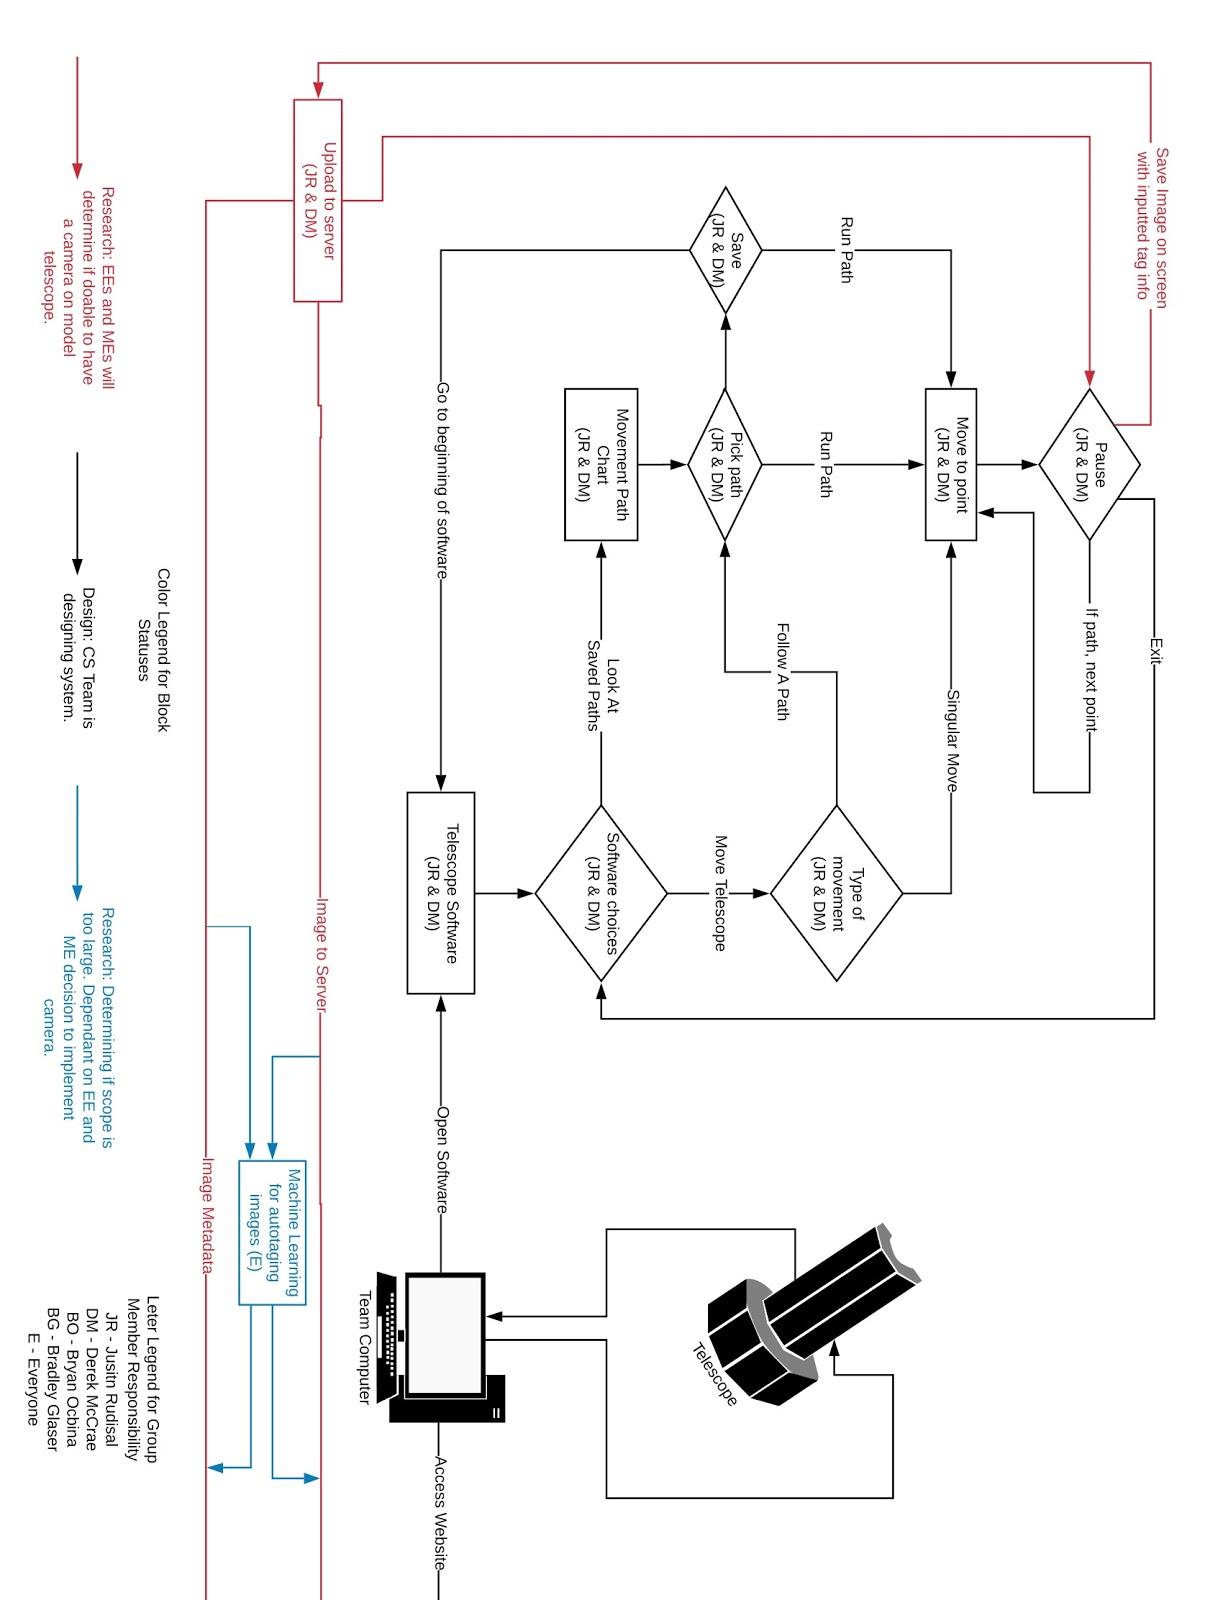
\includegraphics[height=\textheight,width=\linewidth]{blockpt2}
\end{figure}

\begin{figure}
	\centering
	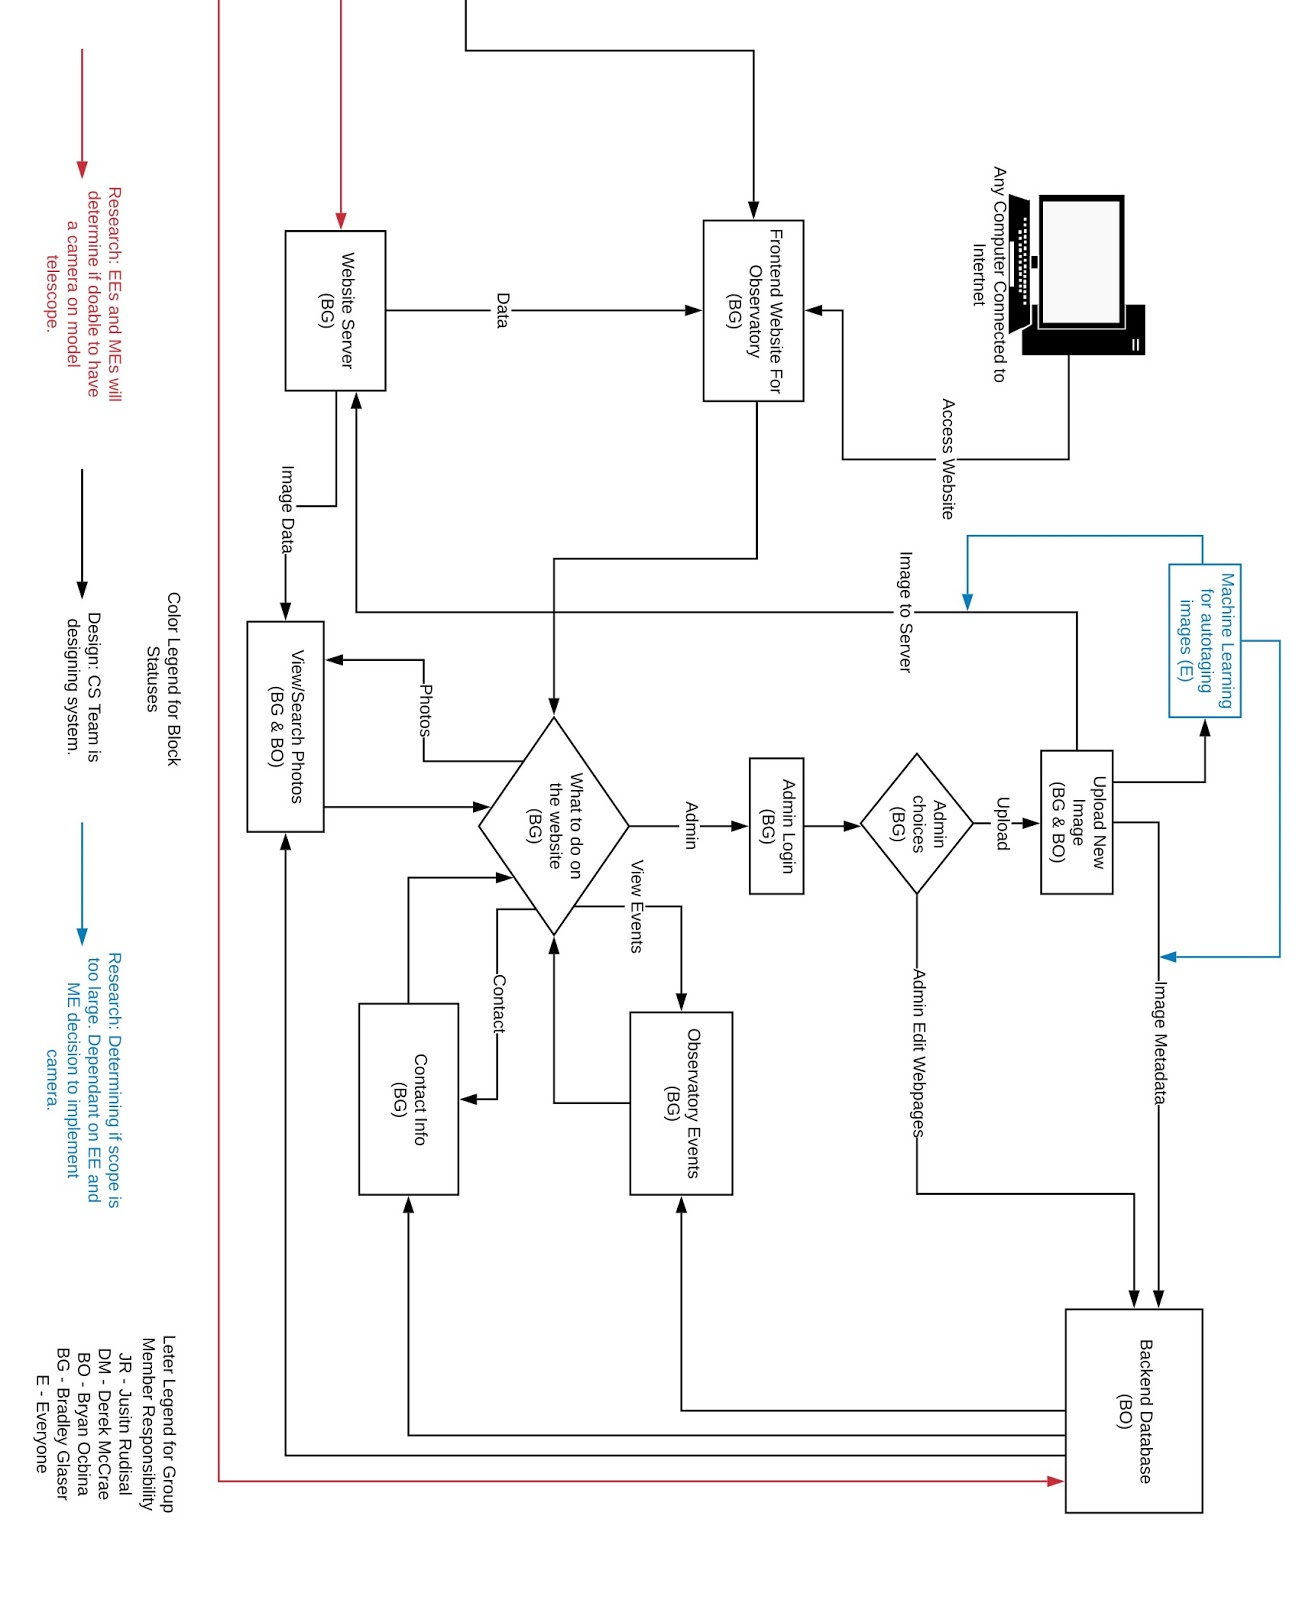
\includegraphics[height=\textheight,width=\linewidth]{blockpt1}
\end{figure}

\newpage %Page break

\begin{figure}
	\section*{Project Milestones SD1}
	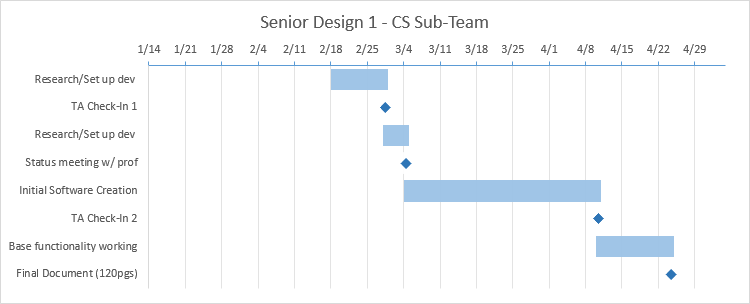
\includegraphics[width=\linewidth]{SD1Gantt}
\end{figure}

\begin{figure}
	\centering
	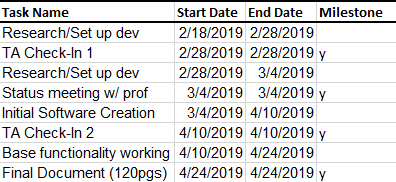
\includegraphics{SD1Dates}
\end{figure}

\clearpage

\begin{figure}
	\section*{Project Milestones SD2}
	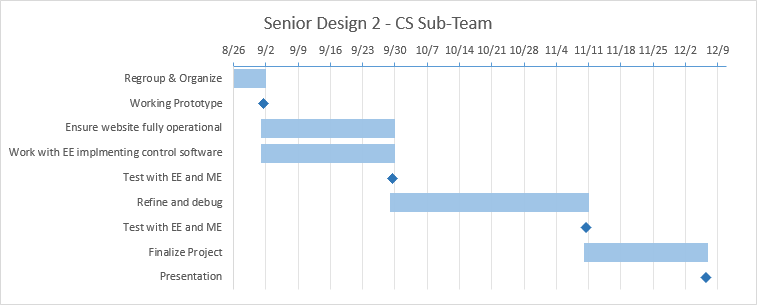
\includegraphics[width=\linewidth]{SD2Gantt}
\end{figure}

\begin{figure}
	\centering
	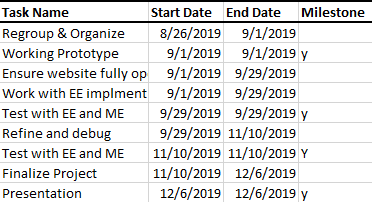
\includegraphics{SD2Dates}
\end{figure}

\clearpage

\section*{Archive Frontend}

The data gathered by the telescope will need to be accessible by future researchers. Likewise, it might be possible to allow the general public to have access to the data. Either way, the data archive will require a frontend to enable browsing, searching, uploading, downloading, and categorizing the data. The frontend will be a login secured website in order to maximize portability and accessibility. By foregoing a native application, we ensure that the data will be accessible from anywhere with an internet connection. Likewise, we enable the researchers to utilize whatever person computers are most convenient. i.e. laptops, a tablet, an iPad, a cell phone, etc.

Figure \ref{fig:archiveusecase} shows a high level overview of the archive frontend. Each action of the archive system performs modifications in the database when they are accessed by the end-user. The actions will be accessible via the interactive website or via the API directly. This separation of function will enable us to potentially expand our project scope as needed. There may be other applications that can utilize the API as part of our project or future projects.

\begin{figure}[h]
	\centering
	\caption{Archive Frontend Use-Case}
	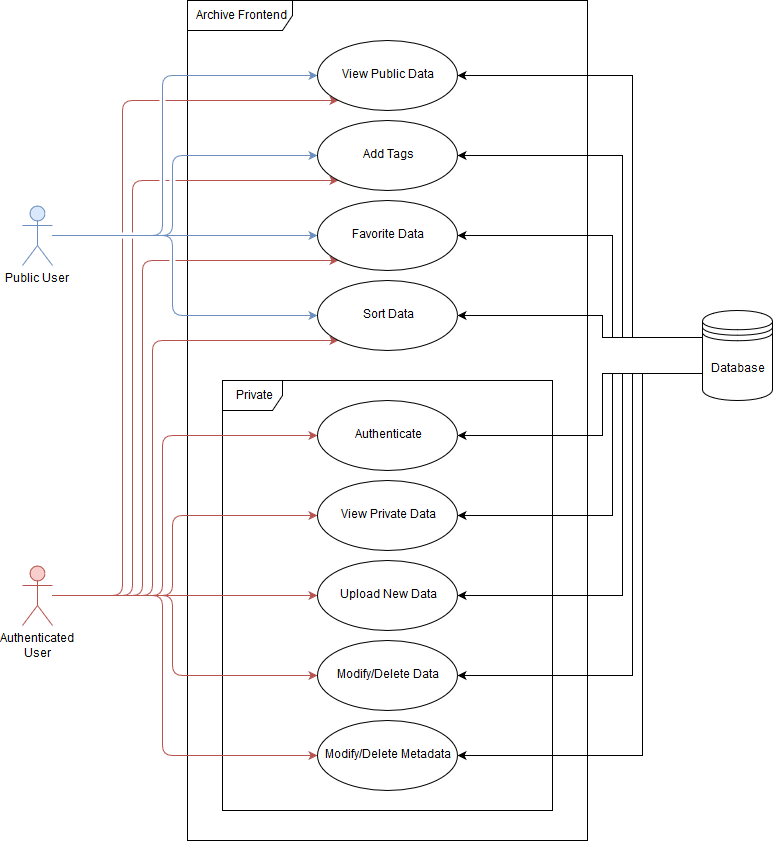
\includegraphics[width=0.75\linewidth]{frontend_use_case}
	\label{fig:archiveusecase}
\end{figure}

The archive will be split into two separate components. Access to the private portion of the website functionality will require logging-in so that the user can be authenticated. Likewise, different users may have access to different sources of private data depending on the security needs of the observatory.

Unauthenticated users will be able to browse the data published as public. We enable said users to perform basic browsing and searching as one would expect. Likewise, we will enable users to add tags and favorites to data. Said information will be stored in the user's cookies until they decide to create an account. Once an account is created, the data stored in their cookies can be uploaded to ensure that the data is persistent across browser sessions.

Authenticated users with the appropriate account permissions will have access to further functionality beyond the basics. They will be able to modify the database directly by uploaded new data and modifying the metadata associated with data that exists withing the archive. Any modifications made by an authenticated user will only apply to data within their permission group. Data may be shared across several permission groups and thus users will only see the modifications made associated with their group. In order to facilitate said functionality, we will need to keep modifications separate from the source data in our backend.

\subsection*{Frontend Frameworks}

Frontend frameworks have become the de facto standard of the web. Industry has moved away from static HTML websites in recent years. Users demand a high degree of interactivity from their websites. Thus, industry has responded by adding more client code in order to facilitate said demand. By utilizing a framework for our project, we will gain vital industry experience that employers are looking for from their applicants.

We opted to utilize a frontend framework in order to facilitate a high degree of interactivity. There are several options for delivering static HTML pages with minimal client-side JavaScript. However, we want to ensure that our client interactions are extremely fast to load. Specifically, sorting data can be offloaded to the client to ensure that one doesn't have to load a new web-page each time that one changes a search parameter. Utilizing a frontend framework enables us to update the data display instantly when said parameters are changed.

There are many modern frontend frameworks which enable developers to quickly create highly interactive websites efficiently. Our frontend solution will need to be data efficient to reduce the strain on potentially poor connections. It is possible that potential users will have a poor internet connection while attempting to access the data. (As is the case in some observatories.) Thus it is necessary to choose the appropriate framework solution which enables rapid development while maintaining a focus on efficiency.

\subsubsection*{Angular}

The Angular web framework was released by Google in September of 2016.\cite{angularrelease} Angular (also known as Angular 2) was released as a replacement for Angular 1. Its release focused on "a wide range of use cases,...[optimization] for developer productivity, small payload size, and performance."\cite{angularrelease} The framework was built from the beginning via "collaboration with the open source development community."\cite{angularrelease} Thus it has received input from many different developers to ensure that it is flexible enough for general use.

Angular utilizes TypeScript as its implementation language which helps reduce bugs associated with loose typing. Typescript also brings many features absent from plain JavaScript which can help to reduce developer time. Utilizing a framework which already utilizes TypeScript will be more advantageous than trying to use it with a framework which was not built to support it.

Angular is built utilizing component objects. The Angular official quick start guide states that "components are the fundamental building blocks of Angular applications."\cite{angularquickstart} These components "display data on the screen, listen for user input, and take action based on that input."\cite{angularquickstart} Components are a good way of breaking one's code up into reusable pieces. By compartmentalizing one's code in this way, there is a reduction in the duplication of effort. Likewise, it creates the opportunity to test each component separately from the rest of the overall application.

Angular is a good candidate for our archive frontend. It was designed to be extremely flexible. Likewise, it is a commonly used industry frontend framework. Employers look for candidates with existing knowledge of frameworks. Thus it would be useful for our team to gain experience using such a common library.

\subsubsection*{Bootstrap}

Bootstrap is an open-source framework originally developed at Twitter in 2010.\cite{bootstrapabout} It was originally a closed-source tool for internal use at Twitter. However, it was eventually open-sourced due to its popularity with the internal Twitter developers. Twitter found that "developers of all skill levels [could jump] in without any external guidance."\cite{bootstrapabout}

Like Angular, Bootstrap also includes components. However, the Bootstrap components are focused on the display of data and abstains from opinions about the structure of one's data. This decoupled nature means that utilizing components ensures that applications built with Bootstrap share a common look and feel. Familiar components ensure that potential users are quick to acclimate.

Unlike other frameworks, Bootstrap relies on jQuery to handle its JavaScript integration.\cite{bootstrapjs} Thus, Bootstrap is much less opinionated on the frontend code structure. This enables developers to create their own code idioms and integrate into existing code bases easily. Likewise, Bootstrap is able to be utilized alongside other frontend frameworks. If we chose to do so, we could utilize a framework like Angular and still use Bootstrap to ensure that our look and feel are familiar and consistent for the end users.

Bootstrap's flexibility is both a strength and a weakness. Experienced JavaScript developers will find said flexibility very useful and will be able to structure their code in a familiar fashion. However, our team lacks experience building frontend web applications. Thus, an opinionated framework may become an initial disadvantage. Other frameworks provide a standard way of structuring code and therefore might be more friendly for our team to work with.

\subsubsection*{Ember}

Ember was a JavaScript frontend library released to compete with Backbone.js, SproutCore, Cappuccino, and Dojo.\cite{emberrelease} Many Ember's original competitors have fallen out of the public eye since its release in August of 2012, yet Ember still sees wide adoption even today. Ember was a departure from aforementioned "microlibrary" competitors that were popular at the time of its launch. Ember was different because it focused on "helping developers grapple with the complexity of building 100\% JavaScript web applications."\cite{emberrelease} They did so by "[embracing] the tools that [web developers] were most comfortable with: HTML and CSS."\cite{emberrelease} Thus, Ember was created as an opinionated JavaScript framework which "[helps] you architect large, multi-page applications, but [helps] you to do so without breaking the basic building blocks of the web."\cite{emberrelease}

When a user visits an individual URL in an Ember application the response is handled via an Ember "route".\cite{emberrouting} Routes are how a developer compartmentalizes pieces of their application functionality into reusable components. Thus, it is important to separate one's application based on functionality to ensure that effort is not duplicated among several different routes. Like the other aforementioned frameworks, Ember enables the developer to test individual components by splitting them up into routes.

Ember decouples data from the display routes via objects called "models".\cite{embermodel} Models are a way to adapt the Ember routes to the application's individual data concerns. Thus, Ember provides strong opinions about how one should structure the application's data.

Ember's focus on preserving web browser functionality is definitely an advantage when compared to some frameworks that may cause something as simple as the back button to function incorrectly. Likewise, its opinionated framework style ensures that our team will have a good idea of how to structure our application. However, Ember's rigid structure might be too strict for our purposes. Our team has compartmentalized the web application into frontend and backend sub-teams. Thus, the frontend team needs to be flexible enough to accommodate however the backend structures their data before the frontend interacts with it.

\subsubsection*{React}

React was a Framework developed by Jordan Walke at Facebook. It was originally a propriety framework that they used internally. However, it was later released as an open-source framework at JSConf US.\cite{reactlaunch} It was released in 2013 and thus it is a relatively new framework in the JavaScript ecosystem.\cite{reactlaunch} However, it has seen high adoption rates among developers.

React is a single-page web application framework. It enables the developer to dynamically update the contents of a page as data changes or uses interact. Since the web browser doesn't have to load completely new pages with each action, the resultant web application is very responsive since it only downloads information as it is needed without the need to potentially re-download components repeated on each page.

Components are React's way of splitting your application into reusable pieces. Likewise, Components determine how one structures the data on the user's end. React components "[take] in parameters...and [they return] a hierarchy of views to display."\cite{reacttutorial} The data is tightly coupled to the visual model. React's opinionated nature is ideal for our inexperienced developers. A framework like React that provides not only the tools for creating the UI we need but also provides structural guidance is an advantage over the other options available.

React's structure and idioms are a good contender for implementation in our project. The single-page nature of React makes it ideal for places with low-bandwidth connections such as observatories. Likewise, the tight coupling of data and view provides a good starting point for structuring our code. Finally, React is widely used in the industry and so it would be an advantage for our team to gain experience using it.

\subsubsection*{Vue}

Vue was released by Evan You in 2014 as an open-source JavaScript frontend framework.\cite{vuelaunch} It received immediate attention from various web communities and it has developed significantly since its launch. It is being actively developed and receives regular bug-fixes and stability patches. Despite its relative immaturity, the framework has seen wide adoption due to its progressive design philosophy.

Vue is compartmentalized across several different libraries. The core library "is focused on the view layer only, and is easy to pick up and integrate with other libraries or existing projects." \cite{vueguide} However, Vue optionally has the capability to "[power] sophisticated Single-Page Applications when used in combination with modern tooling and supporting libraries."\cite{vueguide} Vue's flexibility enables it to integrate into many differing use-cases.

Like the other libraries examined, Vue also supports component composition via Vue's component system. This abstraction system is "an abstraction that allows us to build large-scale applications composed of small, self-contained, and often reusable components."\cite{vueguide} They can be nested and pass data from parent to child. Data passing is done via props and a specialized binding syntax.

Utilizing Vue for our project would mean depending on a relatively immature library. However, its lightweight molecularity will enable us to only utilize the components that we need for our project. By doing so, we will reduce both the complexity of our resultant application and the bandwidth requirements associated with loading the libraries. Likewise, the single-page application nature of Vue will also reduce the amount of data being utilized.

\subsection*{Frontend Programming Languages}

JavaScript is a ubiquitous frontend programming language for use in the browser. Recently, it has also gained popularity in the native application domain via Node.js. Node.js is a open-source cross-platform run-time environment which enables existing JavaScript developers to leverage their skills on the backend. However, despite JavaScript's popularity there are several alternatives that seek to eliminate some of JavaScript's intrinsic pitfalls.

\subsubsection*{CoffeeScript}

CoffeeScript is a language that compiles down to JavaScript.\cite{coffeescriptlittlebook} However, "CoffeeScript is not a superset of JavaScript, so although you can use external JavaScript libraries from inside CoffeeScript, you'll get syntax errors if you compile JavaScript as is."\cite{coffeescriptlittlebook} This sacrifice of direct compatibility comes with sever advantages. Notably, CoffeeScript's succinctness means that the developer typically has less code that they directly have to write.

CoffeeScript has many interesting syntactic features that enable developers to express code concepts more succinctly than plain JavaScript. One such feature is comprehensions.\cite{coffeescriptguide} Comprehensions can replace loops in a more readable fashion and read a lot like English sentences instead of code. Comprehensions greatly shorten the amount of code required to express an idea. Many problems that can be solved via comprehensions are common and may occur across many use cases. The overall style of CoffeeScript borrows from languages like Python, Ruby, and Haskell. Thus, it is very readable and has a focus on clean code paradigms. This readability means that code concepts are parsed more quickly by developers and reduces the chance of confusion when reading source code.

CoffeeScript, once transpiled, runs as plain JavaScript in the client's browser.\cite{coffeescriptguide} This transipation process means that CoffeeScript is compatible across the many different browsers that already support JavaScript by default. However, CoffeeScript utilizes modern JavaScript features.\cite{coffeescriptguide} Thus, it might not be able to run on older browsers which lack support for modern JavaScript. The trad-offs between developer features and client compatibility is some that one must consider whenever choosing a language/library for use. However, our rapid development time-frame might benefit from languages that reduce the amount of necessary boilerplate.

The other languages explored are statically typed; CoffeeScript is not. Dynamic typing can be a double edged blade. It enables rapid development which would be a boon for our team. Likewise, since the code is dynamically typed, it is very flexible. This flexibility ensures that code is resilient to changes in the code base that might require massive refactoring otherwise. However, dynamic typing also has a sinister side. Many bugs which are essentially impossible in a statically typed language can manifest in a dynamically typed language like CoffeeScript. Likewise, it is much harder to develop tools for a dynamically typed language. Type inference can bridge the gap somewhat but it does not yield the same fidelity of information that statically typed languages confers. Thus, the resultant tools associated with a dynamically typed language like CoffeeScript are somewhat weakened by the lack of strong types. Tools are a vital part of developing modern software and our team needs all the help we can get. Thus, the lack of extensive CoffeeScript tools are a potential downside that must be considered before our team commits to utilizing it for as our frontend language.

Like some of the less popular frontends, utilizing CoffeeScript in our project would mean taking a gamble on a product that isn't as widely used as other solutions. Maintainers that come after us would need to be able to service the code without being tripped up by a potentially defunct programming language. However, there is an upside. CoffeeScript's features and syntax would mean less lines of code for our team to write. Language expressiveness is an often overlooked feature when planning a project. Utilizing the right tool for the job is an essential part of the planning process.

\subsubsection*{Dart}

Dart is a general purpose programming language developed by Google as an open-source alternative to existing solutions.\cite{dartlaunch} It was designed to be "structured yet flexible" and to "deliver high performance on all modern web browsers and environments ranging from small handheld devices to server-side execution."\cite{dartlaunch} It was launched by Google in 2011 and has seen varied adoption across different use-cases.

Like the other options explored, Dart can also be transpiled to JavaScript for execution in modern web browsers. It even benefits from compile time optimizations that can, "in some cases, run faster than equivalent code hand-written using JavaScript idioms."\cite{darttalk} The compilation process eliminates the need for some checks and operations that would otherwise need to be performed at run-time. Thus, the resultant code is very fast indeed.

Dart also features prominence in the mobile application space. Google has developed their Android/iOS alternative Flutter for use with the Dart programming language.\cite{darthomepage} Dart runs naively on x86 and ARM computers. Likewise, it also supports a run-time environment with a built in garbage collector and a mature set of core libraries to ensure rapid, safe development of mobile applications. Utilizing Dart for our frontend code would mean gaining a unique skill-set applicable to a blooming mobile application space.

Dart is statically typed with a focus on object-oriented design paradigms. Its syntax was strongly influenced by existing programming languages such as C, Java, C\#, and JavaScript. Thus, it is a highly approachable language that should feel familiar to most developers. This ease of adoption is important for the rapid acclimation of developers on a project. Likewise, it would behoove our team to use a language that is easy to pick up and use due to our limited development time.

Like the other languages explored, Dart has a unique set of tools associated with the language. One such feature is the code analyzer. Its use before deployment can catch bugs before they become an issue in production code. For instance, said analyzer will be able to detect if you fail to cover all possible cases when utilizing enumerations in a switch statement. This small reminder seems trivial at face value but it can cause a lot of headaches if the developer doesn't anticipate it in advance. Likewise, it enables the developer to add new enumeration values without fear. This can be done because once one adds the new values, the analyzer will alert the developer to all the switch statements that need to be modified to include the new enumeration values. Tools like the Dart analyzer are a strong motivation to choose a language alternative to plain JavaScript. Given our teams relative inexperience, we would greatly benefit from such tools and our resultant code will be better as a result.

Utilizing Dart in our frontend would also mean relying on yet another library. Dart has strong opinions about code structure and static typing. Thus, we would need to utilize a middleware library to act as a bridge between our Dart code and whatever frontend library we choose to utilize for implementation. It is possible that any of the libraries that we choose to implement our project may become unmaintained and fall into disuse. Reliance on yet another library reduces the maintainability of our project if future senior design students are tasked with updating, maintaining, or expanding our code. Such an eventuality must be considered before we include yet another library in our project.

Dart represents the unique opportunity to be at the forefront of Google's vision of future application development. It is possible that the mobile market will shift towards a uniform platform like dart in the future. Our team would benefit not only from Dart's feature set but also its potential as a future resume boost. Likewise, given that the language is backed by Google, it is unlikely that it is going to be abandoned like less mature options might. Dart is a strong contender for use in our application frontend.

\subsubsection*{TypeScript}

TypeScript is an open-source programming language released and developed by Microsoft. TypeScript is a syntactic superset of JavaScript that adds optional typing to the language.\cite{typescripthomepage} It is well maintained and under active development.

TypeScript is a very approachable language for both beginners and JavaScript veterans. Its syntax is very familiar to developers who have worked on frontend applications. Thus, it will be very easy for team members to acclimate to the language and become productive quickly. Likewise, it will be advantageous to be able to show code samples to individuals already familiar with JavaScript with minimal friction. Communicating code examples to external individuals is a vital part of presenting one's work. It is important that the language does not increase the cognitive load of the listeners when trying to present new information to them.

TypeScript comes with many tools that aid in the development process. Developing code is hard and it is made harder when tools are unable to assist in the development process. Plain JavaScript's dynamically typed nature limits the functionality of external development tools. However, TypeScript does not suffer the same issues because of its optional static typing. Likewise, TypeScript's tools are able to utilize type inference to bridge the gap between dynamic objects and its statically typed ones.\cite{typescripthomepage} Tools are able to utilize this type inference to display additional information and catch potential run-time bugs before they become an issue.

Like the other alternative languages explored, TypeScript implements additional features not native to plain JavaScript. For instance, TypeScript adds iterators and generators. Modern JavaScript has also implemented safe iterators for arrays. However, if one is attempting to target older browsers, then many new JavaScript features may have to be omitted. TypeScript lacks this problem since the new features will compiled to plain JavaScript index iteration. This means that a developer is able to utilize time-saving features while still supporting older browsers. Reducing developer frustration while maintaining compatibility is a strong motivator for our team to choose TypeScript.

TypeScript is a very strong contender for our frontend implementation language. It has a history of very consistent support by Microsoft and its open-source progress can be directly tracked via its repository on GitHub. Likewise, its recent popularity is no fluke. Many modern fronted developers are choosing TypeScript for their projects due to its superior design decisions to plain JavaScript. Utilizing TypeScript in our project would not only increase developer productivity and provide experience with a popular frontend language but it would also mean a reduction in the number of dynamic-type related bugs.

\subsection*{Frontend Technology Selection}

After much deliberation, our team selected React and TypeScript as our technologies for our frontend implementation. We examined the other frameworks in detail and determined that React would be the best fit for us to use. Likewise, TypeScript stood out among the examined languages as an excellent fit for out project.

We selected React as our frontend framework for several reasons. However, one such reason stood out to us as a huge advantage: the fact that React features tight integration with JSX. JSX is an extension to plain JavaScript which enables one to write HTML tags as a part of the code that one writes. By structuring one's code in this way, data and display logic are tightly coupled together. It makes it much easier to reason about how the eventual web page will be displayed when it is render to the client. Likewise, it simplifies the code since the developer doesn't have to perform searching through the markup to find elements before they are modified. This way of structuring a project was very appealing for our team. After weighing the different options, we felt that the use of this technology was too good to pass up. Structuring the project so that code and markup are tightly coupled means that we can point to single source files when collaborating between team members. Likewise, code review can be extremely modular since the source for an individual component is all contained in one file. The use of JSX was a major contributing factor to our decision to utilize React.

React's focus on efficiency is very compelling. React utilizes the virtual Document Object Model (DOM) to ensure that updates to the visual DOM are only performed when it is absolutely necessary. Hardware in observatories can be very limited in performance. We wanted to ensure that whatever framework we utilize, we focus on delivering an efficient and lightweight user experience. Initial research into the differing frameworks highlighted React as the best contender that fulfilled said requirement. The combination of utilizing JSON API calls and efficient DOM updates will ensure that our web-app performs well enough that observatory researchers are able to utilize it without worrying about performance. This was a very high priority for our team since we envision researchers utilizing our application as an integral part of their daily routine. Any issues regarding performance would severely reduce the likelihood that researchers actually utilize our tool. People are very unlikely to use a tool if it doesn't "feel" good doing so.

React integrates extremely well with TypeScript. The TypeScript website has a section dedicated to getting started with React.\cite{typescriptreacttutorial} Likewise, the React website features a similar tutorial.\cite{reacttypescripttutorial} Therefore, it was our conclusion that integration between the TypeScript language and the React framework would be painless. Our conclusion was reinforced by the existence of type annotations for all necessary React classes and components. Thus, we held a high degree of confidence that we would be able to exploit the advantages that come with using a typed language.

Dynamically typed languages are a liability to the stability of our eventual product. Our frontend website must be able to stand the test of time without unnecessary downtime or fatal bugs that might interrupt the workflow of our eventual users. Our team will not be around to perform maintenance on the archive frontend after we have long since graduated. Thus, in order to reduce the chance that another senior design time will have to come in and clean up our mess, we are avoiding the dynamically typed language JavaScript. We did not make this decision lightly. It is obvious that JavaScript is the industry standard for interactive websites. However, we believe that we will see better stability by supplanting its use via TypeScript.

Typed languages eliminate an entire class of bugs and reduces the frequency of run-time crashes. Research performed by Zhang Gao \textit{et al.} at The University Collage London and Microsoft demonstrated that the use of TypeScript enables developers to reduce the number of bugs by approximately 15\%.\cite{typescriptpaper} They examined the commit history of several open source JavaScript applications. The identified the commits that corresponded to the introduction of a bug. Then, they would leverage TypeScript by adding type annotations to the code in question. If the newly annotated code prevented the bug at compile-time, then they determined that TypeScript would have prevented said bug from ever causing an issue in the first place. Of the 400 public bugs that they examined, TypeScript was able to prevent 58 bugs from occurring due to type checks at compile-time. Their conclusions are really and understatement on the impact of strict typing. They only examined public bugs and thus they did not account for bugs that were caught by developers manually during the development process. Likewise, strict typing also impacts the quality of the tools surrounding a language. Simple tasks in code navigation suchas "go to definition" and "see usages" are substantially improved by strict typing. Similarly, strict typing can reduce developer confusion since the arguments to a function or method include additional information beyond simply their name. i.e. the types associated with the arguments passed to the method in question. The results of the Zhang Gao paper was a huge motivating factor for our team. We are not expert frontend developers and thus we benefit from the additional power that TypeScript brings during the tooling process.

\subsection*{Extended Frontend Research}

Before we can begin planning the structure of our frontend code, we must first take a closer look at the way that React applications are built. This section examines many of React's idioms, components, props, application state, application life-cycle, and fillable web forms. Understanding how each of these elements make-up a React application will give our team the groundwork to begin creating our own React application for use in the archive system. It is vital that our team has a good understand of how a React application functions before we begin implementation due to our constrained timeline. Likewise, utilizing React idioms appropriately will ensure that future senior design students who might maintain or extend our code will be able to have an appropriate starting point for their project. The last thing that our team wants is to deliver a project that will just have to be scrapped and rewritten if/when any future maintenance is needed.

\subsubsection*{A Closer Examination of React Components}

Components are the main way in which one structures a React application. As mentioned above, components are React's way of compartmentalizing reusable pieces of one's design. They can be structured as side-effect free functions or as classes which extend the \texttt{React.Component} super-class.

Functional components are a good way of structuring simple components. They fit when a component doesn't have a need for child components or if its child components don't have a need to access the parent's props. Figure \ref{fig:reactfunctionalcomponent} shows a simple React functional component.\cite{reactcomponentsandprops} React automatically calls the function as needed when the associated prop data changes. This leads to very efficient rendering and simple code structure.

\begin{figure}[h]
	\centering
	\caption{React Functional Component}
	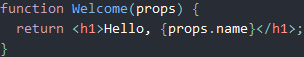
\includegraphics[scale=0.5]{react_functional_component}
	\label{fig:reactfunctionalcomponent}
\end{figure}

Class components are the heavy lifters in the React framework and typically make up the majority of the components implemented. The class components enable the developer to encapsulate the functionality of a piece of the web application to ensure that it is reusable. Likewise, utilizing class components keeps all of the necessary data associated with the markup being rendered. This structure ensures that any callbacks such as \texttt{onClick} can be swapped out since they can reference the properties of the encapsulating class. Click handlers can by dynamically assigned depending on the application's current context. This flexibility enables the developer to write generic components which can be reused and repurposed.

\begin{figure}[h]
	\centering
	\caption{React Functional Component}
	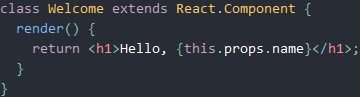
\includegraphics[scale=0.5]{react_class_component}
	\label{fig:reactclasscomponent}
\end{figure}

\subsubsection*{How React Handles State}

React handles state via prop objects. Props are arbitrary inputs that are passed to React components at run-time. The data contained within said props is the used to update the display to the end-user.

Props are read-only and cannot be directly modified. This invariant is not enforced by the library and must be strictly adhered to by the developer. Direct modifications to a prop can cause very strange behavior and possible bugs or even crashes. Instead of direct modification, props are updated via the \texttt{setState} method. This method is inherited from the \texttt{React.Component} super-class that all React components must inherit from. Utilizing \texttt{setState} instead of direct modification enables React to update the browser Document Object Model (DOM) lazily. This lazy update technique is at the core of what makes React a fast and efficient framework.

Frontend applications are asynchronous by nature and React is designed to accommodate async behavior by its very nature. Frontend applications must utilize async methods to ensure that the user experience is unaffected by long-running tasks such as network calls. There are many methods of accomplishing asynchronous dispatch but React is equipped to handle any of them provided that they adhere to the state invariants that React mandates. The \texttt{setState} method mentioned above enables React to accept statue updates from async sources and update the visual DOM efficiently. The \texttt{setState} method can merge several state updates into the existing component state in a batch fashion. Like the other React design decisions, the asynchronous allowances provided by the \texttt{setState} method are done for the state of efficiency and lazy evaluation.

Data in a React application always flows down. Parent components are able to update the state of their children. However, the reverse is not true. This unidirectional flow invariant also contributes to the lazy update technique discussed above. By ensuring that the data only flows in one direction, React can eliminate the need to update entire branches of the DOM.

React components are unable to tell if their children are stateful or stateless. i.e. class components or functional components. This separation of concerns contributes to the modularity of React components. Data is passed from parent to child and since data modifications are only performed via prop updates components can be refactored without great difficulty.

\subsubsection*{Asynchronous Data Fetching}

In order to build applications that feel responsive, asynchronous HTTP requests are a necessity. Executing requests on the rendering thread is a surefire way to make one's application feel sluggish given the nature of computer networking. Users are accustomed to instant feedback for their actions. As previously mentioned, React is quite happy to accept updates from asynchronous sources. However, like the other technologies examined, industry has moved away from utilizing plain JavaScript to handle HTTP requests. It is perfectly viable to perform said requests in plain JavaScript but there a plenty of libraries which exist to simplify the process and reduce the chance for errors. We briefly examined three methods of executing HTTP requests: plain JavaScript, the Request library, and the Axios library.

Utilizing plain JavaScript for HTTP requests cannot be overlooked. Our project will need to make simple HTTP REST requests. JavaScript is perfectly capable of handling said requests without any additional library requirements. Given that our project might need to maintained by other individuals or students in years to come, it would behoove us to attempt to minimize the number of libraries that must be learned before they can get started making modifications. Figure \ref{fig:javascripthttprequest} shows a simple HTTP request snippet provided by the Mozilla developer documents.\cite{mozillahttprequest} The aforementioned snippet shows that JavaScript is perfectly capable of making asynchronous requests in an idiomatic way. The developer just needs to declare anonymous functions to handle the callbacks which will be fired when the request completes.

\begin{figure}[h]
	\centering
	\caption{Plain JavaScript HTTP Request}
	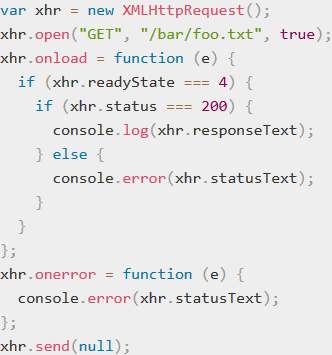
\includegraphics[scale=0.5]{javascript_http_request}
	\label{fig:javascripthttprequest}
\end{figure}

Request is a popular JavaScript library for handling HTTP requests in a simplified manner. It condenses the verbose syntax required for plain JavaScript HTTP requests into a specialized set of functions with sane defaults. Some such convenient helper methods are: \texttt{request.get()}, \texttt{request.post()}, \texttt{request.put()}, etc. Since HTTP request code is repeated in several places, it is beneficial for a developer to utilize a library with a clean and friendly syntax to reduce the chance that a mistake will be made when constructing the HTTP request code.

\begin{figure}[h]
	\centering
	\caption{An Example of the Axios Library Usage}
	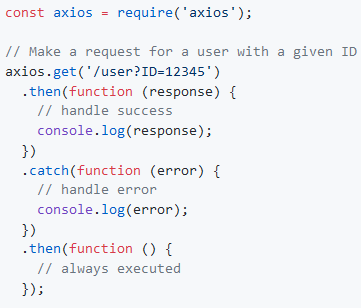
\includegraphics[scale=0.5]{axios_example}
	\label{fig:axiosexample}
\end{figure}

Axios is another well known JavaScript HTTP client library that seeks to simplify the process of making HTTP requests. However, unlike Request, Axios puts a focus on utilizing the promise API to manage its connection responses. Thus it requires a modern version of JavaScript (ES6+) in order to function. However, despite this limitation, the resultant code one writes when using Axios ends up being very clean and understandable. Figure \ref{fig:axiosexample} shows an example of utilizing the Axios API to make a basic GET request corresponding to a specific userID.\cite{axiosgithub} The example code provided shows the power of chaining several Axios methods together. The example code is very readable and mirrors the structure of natural language instructions. Structuring code in this way helps to reduce the cognitive load on the developer. This leads to better code and faster code reviews since it is easier to explain to other developers what each method call accomplishes.

\subsection*{Frontend Design}

In order for our archive to be actually useful, it must be more accessible and specialized than a simple file browser. It must serve the needs of the individual researchers at the observatory and simplify their workflow in order to magnify their productivity. Thus we will utilize the metadata contained within the Flexible Image Transport System (FITS) file format. In doing so, we will enable the researchers to search and categorize data without the need of opening individual files to inspect the associated metadata.

The Flexible Image Transport System (FITS) file format is a well known file format in the astronomy community. Much of the data generated by observatories are contained within FITS files. Our research indicates that there are many open source libraries for interacting with FITS files. However, native file browsers lack access to much of the data contained within. Thus, searching for and organizing the data is constrained by the native file browser's limitations. We seek to extricate the metadata out of the individual FITS files and create a database that can be queried for the metadata in a dynamic way. The archive frontend will need to utilize the backend API to display the metadata to the end user as they browse the archive's contents. By organizing our application in this way, we minimize the amount of data that needs to be sent by the server since not all of the metadata is needed in order to display the files as one browses the archive's contents.

Figure \ref{fig:frontendmockup} shows a mock-up of the archive's homepage. It will serve as the hub for browsing the archive's contents. The decision to display data on the homepage reflects our commitment to simplifying the access to the observatory's data. As previously mentioned, it is vital that researcher's have quick access to the data contained within the archive. Our hope is that the archive website becomes an invaluable part of their daily workflow. Navigating through a user interface before one even gains access to the data is counter-productive to that end goal.

\begin{figure}[h]
	\centering
	\caption{Mock-up of the Primary Frontend Homepage}
	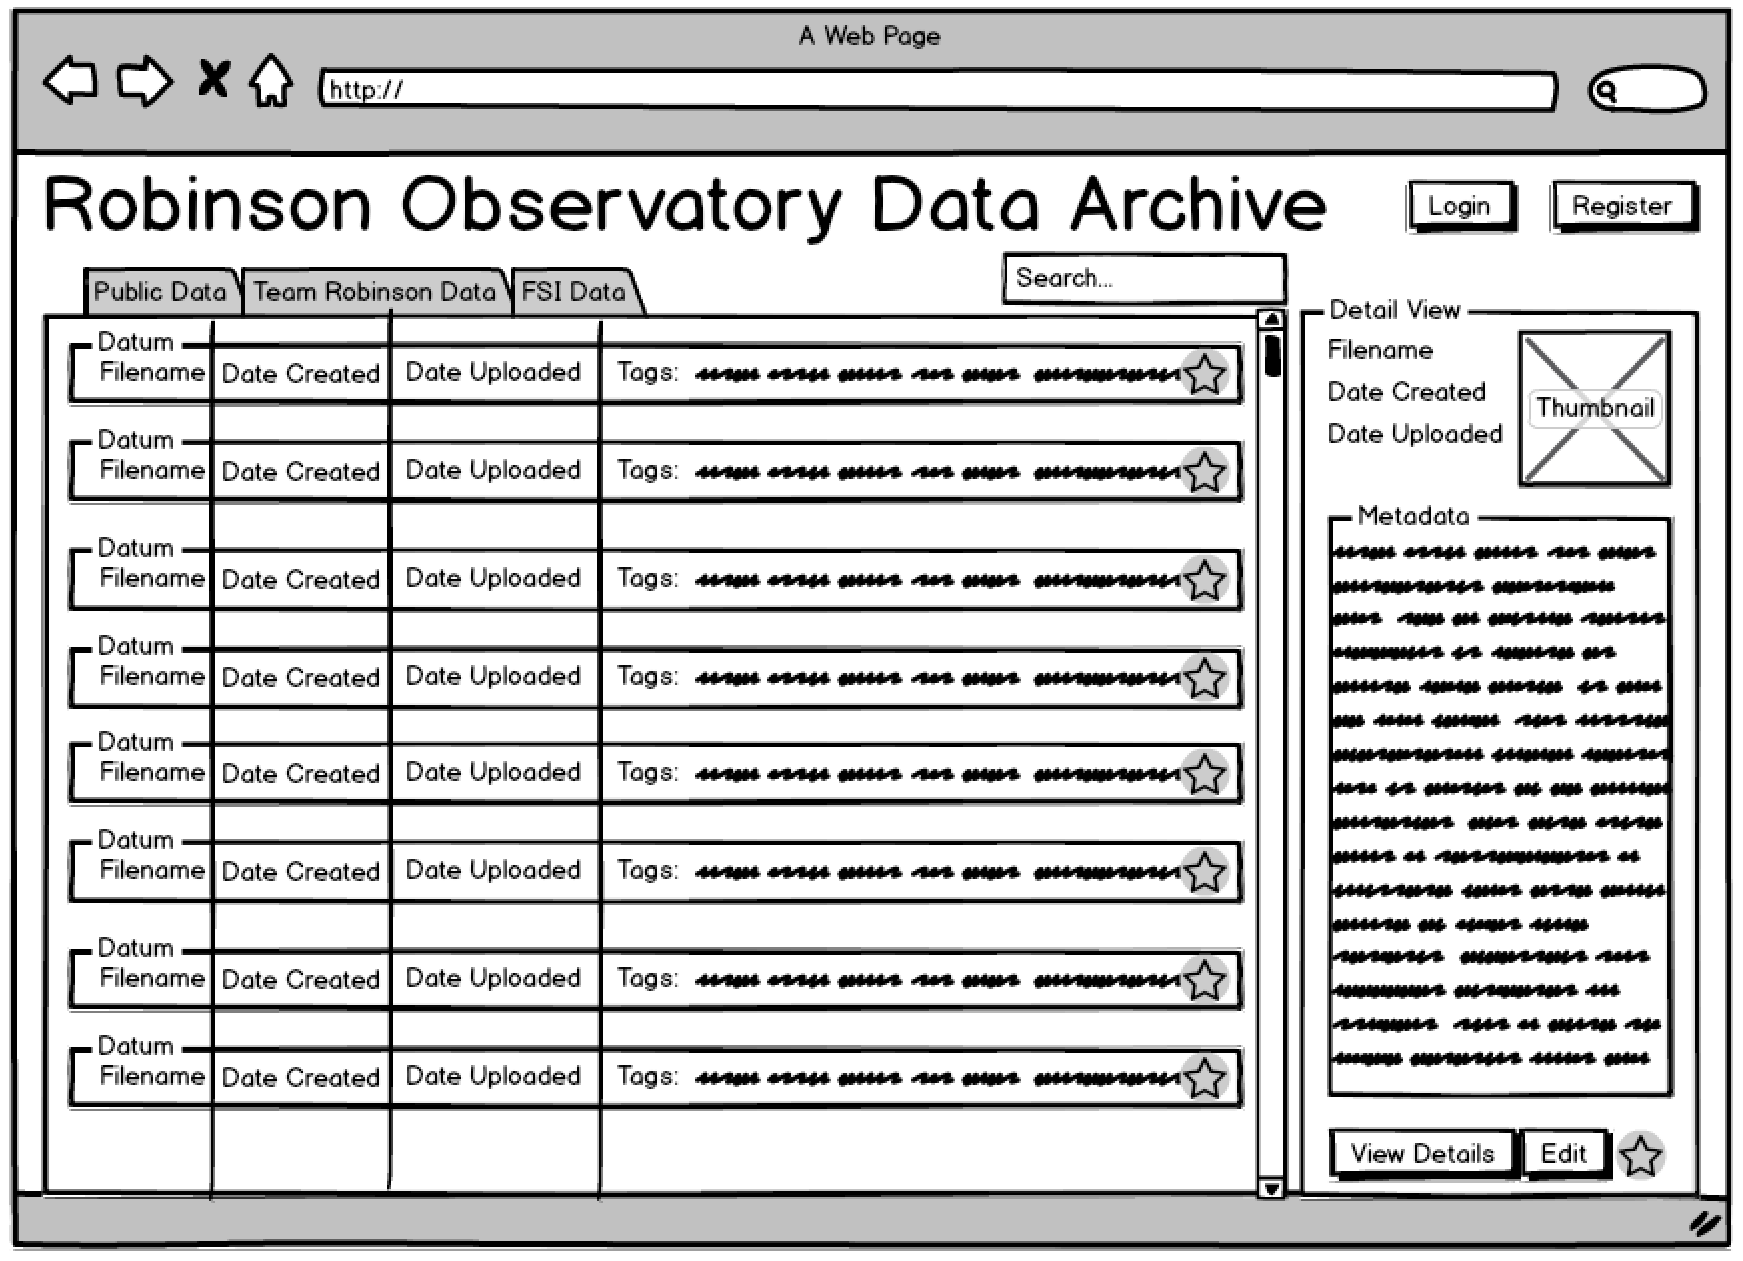
\includegraphics[width=\linewidth]{frontend_mockup}
	\label{fig:frontendmockup}
\end{figure}

\subsubsection*{The Archive's Splash Screen}

Displaying data as the first thing that one sees may be initially jarring to someone unaccustomed to the website. Thus, it may be prudent to display a splash screen message when one visits the website for the first time. This would serve to ease the user into the system and help to prevent them from being overwhelmed with options. Such a splash screen would then be disabled upon subsequent visits to the archive. Figure \ref{fig:splashscreenmockup} shows our initial designs for a splash screen that would be displayed to first time visitors.

\begin{figure}[h]
	\centering
	\caption{Mock-up of the Welcome Splash Screen}
	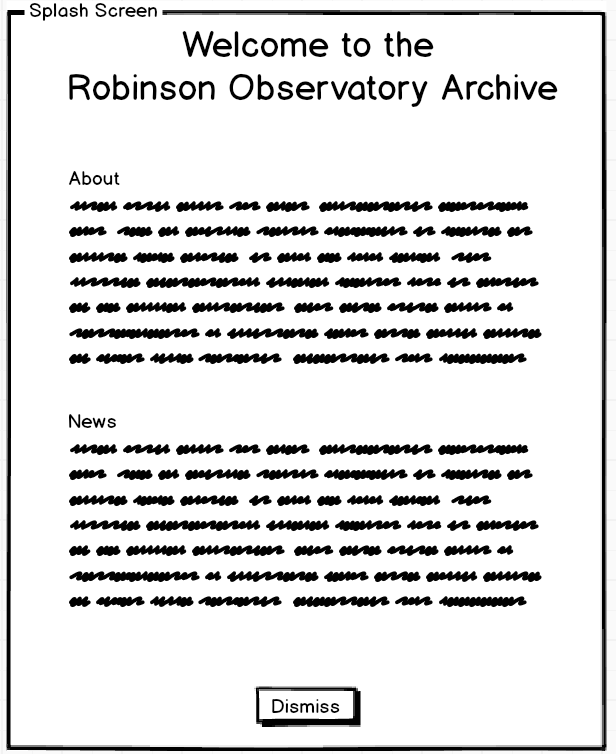
\includegraphics[scale=0.33]{splash_screen_mockup}
	\label{fig:splashscreenmockup}
\end{figure}

The splash screen would explain details about the archive's purpose and information about the observatory in the about section. We want the about section to answer questions that both the public might have and information that would be useful for researchers. Thus it is vitally important that the information contained within the about section is sourced from both researchers and unprejudiced members of the general public. We will need to interview researchers and the public in order to construct the about section's content. It is vital that this portion of the website is well constructed since it is very likely that it will be the first thing that a user reads upon visiting the archive. First impressions are vital to user engagement. A potential spelling or grammar mistake in this section could color a user's impression about the archive in a very lasting and impactful way.

Another section of the splash screen could display news about community outreach projects that the Robinson Observatory team are currently involved in. Likewise, the news section can contain links to said information so that first time visitors are exposed to the other websites that the Robinson Observatory maintains. This would also help to mitigate the impact on users that potentially stumble on the archive unintentionally. It would provide them with a convenient escape-hatch which would take them back to the "friendlier" (i.e. community focused) portions of the observatory's web-presence. This section is tightly connected to the about section since it is also might be the first thing that one reads in the archive. However, since it is the second thing displayed, readers are likely to be somewhat engaged if they stuck around to get to this section. Thus it is possible for use to include potentially denser content since the fact that they are reading the section means that they are more interested than the casual visitor might be.

\subsubsection*{The File Browser}

Once the user dismisses the splash screen, they are presented with the primary interface. As previously mentioned, Figure \ref{fig:frontendmockup} shows the general layout of the archive home page. The left-hand side of the page will display the the data which has been uploaded to the archive. Internally, we have been referring to this section as the \textit{file browser}. It will function similarly to a standard operating system file browser. However, it will be augmented with the capacity to sort and search based on the FITS file format metadata. Likewise, we want to be able to support custom tags which will simplify the process of working with the data during research.

The file browser will need to be paginated due to the high likelihood that there will be a large number of files uploaded to the archive. Downloading an entire list during each visit would be unnecessarily bandwidth intensive. There are two approaches that we have considered and will need to be experimented with as we begin implementation. The first is a standard pager layout with arrows at the top/bottom of the file browser window. This will enable the end-user to move along as they exhaust their search. This approach is practical and familiar to the average user. Likewise, this is the strategy that Google utilizes for their search queries. (The fact that Google uses this for their interface is a good indication that we should utilize this approach.) Another alternative is to dynamically load new data as the user scrolls in an attempt to make the scrolling as seamless as possible. However, this strategy comes with a fair amount of additional technical requirements. The client must be able to detect which direction that a user is scrolling and dynamically cache the required information in the browser. This is a complex technique that would add a significant amount of difficulty to our implementation. However, if done properly, it would significantly increase the satisfaction and usability of our archive frontend. It would help to convince the end-user that the data is immediately available and it would help to reduce the perception that the data is stored on an external server. It is our belief that making the data seem like it is immediately available will increase the likelihood that a researcher would be satisfied while utilizing our archive. Any perceived delay might cause a potential user to manually cache the files that they are working with. We want to discourage such a practice by making our archive workflow as seamless as possible.

\subsubsection*{The File Preview}

Navigation of the archive is only one aspect of the archive. The second and perhaps more obvious aspect is the need to view the files directly. Research cannot be performed on the data if it is unable to be viewed. Thus we need to be able to display the data within the archive as the end-user searches. We have explored several options for displaying the data as one performs the search.

The first, and perhaps most obvious option for displaying the data, is to enable the end-user to navigate to a details page upon selection of an entry in the file browser. However, this strategy is somewhat counterproductive to our goal of simplifying the user's workflow. Switching context as one searches would interrupt one's thought process. It would be akin to going into another room when one turns the page in a book. Each file inspection would not only switch the context of the web-browser but also the context of the end-user's brain. There is a reason that integrated development environments (IDEs) have so many sub-views displayed on screen at the same time. Switching context inherently interrupts one's thought process. Another aspect to consider is the preservation of application state between context switching. As previously mentioned, we plan on utilizing React as our frontend framework. It is quite possible that, given React's nature as a "single-page frontend framework", we will have to implement some additional logic to ensure that the end-user is able to return to the exact scroll-position upon navigating back from the aforementioned context switch. This additional complexity might save memory on low end computers since we would be serializing the state to disk but this advantage seems somewhat negligible in the face of additional complex code requirements. Thus, this option is unappealing despite its conceptually simple nature.

The second option that we explored for displaying the contents of each file is a always visible file preview sidebar. Figure \ref{fig:frontendmockup} demonstrates this design on the right side of the preview browser display. It is always visible and serves to display the contents about the currently selected file as one scrolls through all files in the archive. This approach ensures that the user's workflow is not interrupted by a switch in context. The pertinent data is always displayed on screen and so the user only needs to look to the side to determine if it is the file that they are looking for. The obvious downside to this approach is that screen real estate is always a concern when one is designing a user interface. Smaller screens will need to be able to display the maximum amount of data on the screen at a time. Likewise, this approach would severely hamper our ability to display the archive on mobile browsers. It is very likely that the file preview would come to dominate the entire screen on such devices. This would mean that our archive would either be unsuitable for mobile devices (an unattractive proposition since one of our stated goals is accessibility) or we would need to adapt our design to remove the preview sidebar when it detects a small display. The latter is an attractive option and would been potentially easy to implement. However, a loss of functionality, no matter how necessary, is something to be lamented. Yet trade-offs must be made and we suspect that mobile users are willing to accept said trade-offs provided that they have access to the requisite data. Thus, the file preview sidebar is a very attractive option for our purposes.

The final option that our team has explored is a floating detail display view. Figure \ref{fig:frontendfloating} demonstrates this alternative layout as a modification on Figure \ref{fig:frontendmockup}. This option is something of a middle ground between the two prior options. Upon selecting a file to preview. The floating view would be presented to the user in the foreground of the current display. Elements from the active file browser would still be visible but partially obscured by the floating view. This would mean that current context would not be entirely lost by navigating to a new page entirely. Likewise, as previously mentioned, the end-users brain context would not be completely lost by a complete swap in visual information. The new information would be "anchored" by the prior view in the background. The extra screen real estate taken up by the floating view would mean that would be able to display more of the data's metadata on screen at a time. This would reduce the need for a scroll-bar attached to the metadata section. It is still possible that one will be required depending on the quantity of metadata present. However, displaying more at a time would imply that the user could find what they are looking for more quickly. In total, this display strategy would hopefully mean that the inspection of files would be a rapid process and that the archive's usability would be greatly augmented by utilizing this strategy.

\begin{figure}[h]
	\centering
	\caption{An Alternative Mock-up of the Primary Frontend Homepage}
	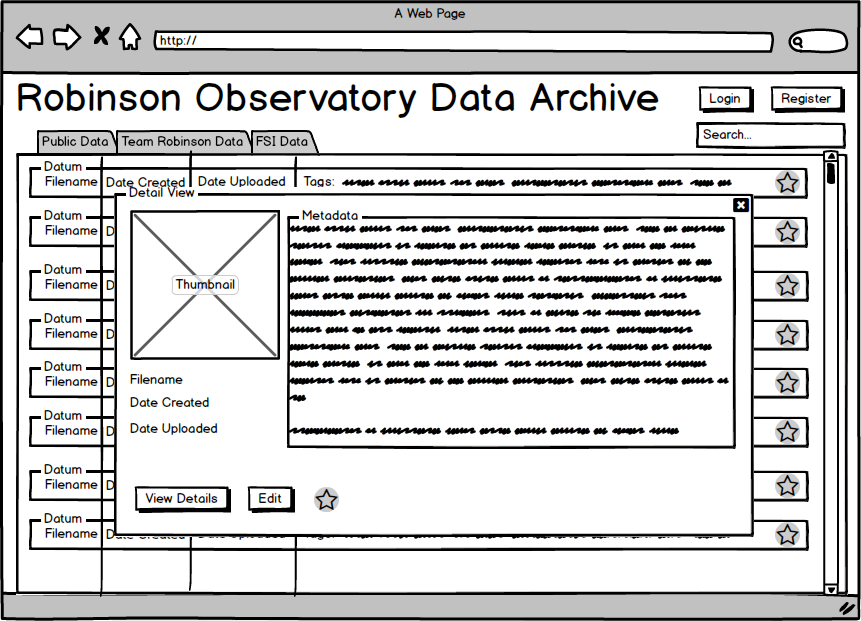
\includegraphics[width=\linewidth]{frontend_floating}
	\label{fig:frontendfloating}
\end{figure}

\section*{Database Research}

\subsection*{SQL vs NoSQL}

\subsubsection*{SQL}

Structured Query Language (SQL) is the most popular language for managing Relational Database Management System (RDBMS).  SQL was initially developed by IBM researchers Raymond Boyce and Donald Chamberlin in the 1970s.  SQL includes data query, data manipulation (insert, update, and delete), data definition, and data access control.  SQL is known for its readability and ease of learning.  MySQL and Microsoft SQL Server are two widely used database systems each being used for LAMP stacks and WISA stacks respectively.  Just recently, both options have become available on Windows, Linux, and MAC OS X.  Due to its age and availability, SQL is heavily documented in its functionality.

\subsubsection*{MySQL}

MySQL is an open source Relational Database Management System (RDBMS) that uses Structured Query Language (SQL).  MySQL is the database component of the LAMP (Linux, Apache, MySQL, PHP) web application software stack.  MySQL is used by popular companies such as Netflix, NASA, Tesla, and Youtube.  MySQL was created by a Swedish company, MySQL AB, by David Axmark and Michael Widenius in 1995 and is currently owned by Oracle.  Similar to SQL itself due to the age of MySQL, its complexity and problems have been encountered and documented so solutions are readily available.  The popularity of MySQL creates a loop of being popular due to its popularity.  Developers are readily available and the cheap hosting environments makes MySQL very accessible.  It is primarily written in C and C++.  While still open source under Oracle, some modules are proprietary and close-sourced.  

\subsubsection*{Microsoft SQL Server}

SQL server is owned by Microsoft and has frequent releases.  The licenses required for running SQL server makes it more expensive than MySQL which is free and open-source outside of the enterprise level.  SQL server is mainly used in Microsoft’s WISA (Windows, IIS, SQL Server, ASP.NET) stacks where all components were designed by Microsoft and built to function together.  The added benefit of WISA stacks is that customer support can be handled by Microsoft across all levels.  SQL server is very to install and has transparent data compression and encryption which also provides better security features. 

\subsubsection*{NoSQL}

A database technology that does not involve the structured query language and rely on object-oriented APIs instead.  NoSQL contains various database types mainly including document databases, graph stores, key-value stores, and wide-column stores.  A document database will pair a key with a complex data structure known as a document.  Graph stores store data based on networks of data e.g. social connections.  Key-value stores store every single item as an attribute name along with its value.  Wide-column stores make use of columns of data, rather than rows.  NoSQL provides a more scalable platform and improved performance.  The various structures of data storage and management alongside cloud development were key features of NoSQL that SQL did not anticipate.  
NoSQL provide dynamic schemas rather than the strict requirements of relational databases.  Adding additional information requirements in relational databases require downtime in shifting all of the previous information to the new tables.  NoSQL and lack of table structure provides flexibility that is unseen in relational databases.  When not all specifications are known or explored in advance, NoSQL is able to add additional data requirements more easily.  NoSQL is developed with cloud storage in mind and is able to easily make use of cloud data storage whereas relational database systems do not support this natively.  
NoSQL Databases are a newer technology from the late 2000s that were developed specifically to combat the limitations of SQL databases, mainly scalability, multi-structured data, geo-distribution, and agile development.  NoSQL databases are widely more dynamic and flexible than SQL databases and remain open source.

\subsection*{SQL Alternatives}

\subsubsection*{MariaDB}

MariaDB was created by MySQL founder Michael Widenius when Oracle obtained MySQL in 2010 and stays true to its open source, community driven development.  MariaDB is a direct alternative to MySQL and is a fork of MySQL.  The functionality is similar enough that MariaDB functions as a database as a drop-in replacement for MySQL.  The database structure and indexes are the same as MySQL.  MariaDB is used by companies such as Google, Wikipedia, RedHat, etc.  The main advantages of MariaDB despite being a fork is its more efficient performance and newer features.

\subsubsection*{PostgreSQL}

PostgreSQL is another open source SQL database but it is object-relational.  Object-relational means that there is support for user-defined objects and their behaviors e.g. data types, functions, operators, domains, and indexes.  Alongside these objects, PostgreSQL has a wide support for data types and structures.  PostgreSQL can store much more data in their rows without negatively impacted performance.  MySQL and MariaDB are known for running into file size limitations and PostgreSQL will avoid those problems.  The highly customizable databases and wide support for programming languages are some key features of PostgreSQL.  PostgreSQL is not as popular as other options but it has many unique features.

\subsubsection*{mongoDB}

MongoDB is the database component of the MEAN (mongoDB, Express, Angular, Node.js) and is a NoSQL database.  MongoDB is based in JavaScript alongside the entire MEAN web-based application stack.  MongoDB was developed in 2007 and introduced to the market in 2009 as an open source database that was maintained and supported by MongoDB Inc.  MongoDB utilizes JSON based document oriented queries that function much more quickly than SQL queries.  NoSQL databases are a more modern approach to databases and mongoDB is in the forefront.  In terms of modernity and future web stack development, mongoDB seems like the most flexible choice for databases.  

\section*{Back-end Research}

The main component for communication between the front-end user experience and the database itself.  The server-side functionality of retrieving and storing data as requested by users into the database and other various API function calls is the job of the back-end.  Mainly consists of the servers, databases, APIs, and operating systems.      

\subsection*{PHP}

PHP began development in 1994 by Rasmus Lerdorf.   PHP is a general-purpose programming language designed for web development and can be easily embedded into HTML.  The PHP code is executed server side which will send the corresponding html to the client.  From personal experience it is somewhat intuitive and relatively streamlined and template based.  Within the PHP code, a connection to the database will be made, a SQL query will be processed from the client and the corresponding data will be sent or retrieved from the SQL database.  The connection will then be closed until the next client interaction happens.   

\subsection*{Node.js}

Node.js is an open source server environment that executes JavaScript on the server and works in conjunction with express.  Node.js differs from PHP as it makes use of asynchronous programming.  Asynchronous programming makes Node.js much more efficient as it is able to send requests and immediately prepare other requests rather than waiting after every single request.  As soon as a request is ready, the contents will be sent to the client rather than waiting for the request to be fulfilled.  The MEAN stack of Node.js will make use of JavaScript across the stack which will provide easier communication across the levels of the stack between developers.  This aspect will be particularly useful in the scope of this project as there are very few of us and communication and ease of troubleshooting is extremely important.

Node.js and the MEAN stack in general is not as mature as technologies as PHP and the LAMP stack but their more modern approach to web development is very promising and the growth in popularity in the last decade is exciting.  Asynchronous calls are more useful in real time environments such as chat systems while not too critical for websites or images but the benefits are there.  

\subsection*{ASP.NET}

ASP.NET is a combination of Active Server Pages (ASP) and .Net Framework.  ASP is Microsoft’s scripting engine for dynamic web pages and .NET is the software that enables use of ASP.  ASP.NET is part of the WISA stack.  The closed source aspect of being a Microsoft product can be a drawback.  WISA stacks and the prices associated seem to be mainly targeting enterprise level websites. 

\subsection*{Ruby on Rails}

Ruby on Rails is a server-side web application framework written in Ruby under MIT license.  Rails provides a model-view-controller (MVC) framework and structures for a database, web service, and web pages.  The frameworks provide a platform and templates for developing websites.  The process with rails seems to simplify the coding process similar to design patterns by providing efficient and clean solutions to common issues or specifications in web application development.  Ruby on Rails sounds like a user-friendly option that could be worth exploring.
 
\section*{Web Hosting}

The current website for the Robinson Observatory is currently maintained by the astronomer team and is apart of the UCF website domain.  This will give us flexibility in what features will be added.  While working on the future additions to the website, we will host the website on our own service.  Image hosting and associated data will be a large component of the website.  Data storage will be a requirement to keep in mind.  The possibility of machine learning being a functionality will increase storage space dramatically.

\subsection*{Amazon Web Services (AWS) vs DigitalOcean vs Google Cloud}

The big three website hosting services are AWS, DigitalOcean, and Google Cloud.  In terms of cost and user-friendly experience in setting up a service, DigitalOcean and Google Cloud seem much more simpler.  AWS offers a wide variety of options and varying levels security or requirements which can make narrowing down your specific needs confusing.  DigitalOcean seems to be the most affordable choice alongside with the medium-scale demonstration size of the website for this project will be.

\section*{Model Telescope Control}

\subsection*{Model Telescope vs Observatory Control}

The underlying premise that drives the need for our model telescope is to replicate the control structure that the Robinson Observatory currently has in a scaled-down and testable environment. The observatory is currently controlled by a software and hardware system known as SkyX Professional, which is a commonly used product for small observatories around the globe that helps individuals get their observatory telescopes operating to their fullest extent. However, while this software is extremely useful for the observatories purposes, it is actually a hindrance for our scale model. SkyX Professional does not translate well when being adapted to small-scale custom designed telescopes. By our understanding based on documentation, as well as the physical systems currently in the Robinson observatory itself, the software has a required hardware integration to use the SkyX software for the purposes of controlling the observatory. 

To further explain, this hardware integration is not designed to be used with telescopes that have been fully planned and created from scratch. The main issue lies in that a custom telescope would have its own custom inputs and outputs based on the needs of the creator, while SkyX and its hardware is designed to integrate with well-established brands and models. The actual SkyX software and what it’s sending out and receiving form the observatory telescope is hidden behind a layer of proprietary silence, and so therein lies the need for a custom model telescope control system. We cannot use SkyX as the observatory currently uses it because we are unable to tell what the software and hardware are communicating to each other beyond our reasoning of what we think it might be sending. 

\subsection*{Designing the Model Telescope Control Environment}

With the realization that we could not go the SkyX Professional route for our model telescope also came the realization that we would have to create our own custom telescope control software from scratch. Before doing any further research into what our software will do and how it will function, we first established as a team that this custom software will be open-source and easily transferable from our scale-model telescope to any real telescope. The idea behind this is that we want to be able to take our software and have senior design teams after us be able to use it as a well-defined base for repairing the Robinson Observatory. The entire thought-process behind the scale model to begin with is due to that fact that there is no currently established base, and so our team has no reference form which to repair the observatory ourselves as it stands. 

After some brainstorming and hashing around ideas, our team established that there would be little difference between our model telescope and a robot. In fact, our telescope would essentially be a controllable robot. With this in mind, we realized that we needed to establish a base software from which to do this controlling from. Taking the stance of this being a robot, we are now also free to design and program entirely within a simulator environment to ensure our software will actually work with the physical custom model telescope.  

\subsection*{ROS Integration with Stand-Alone Gazebo}

\subsubsection*{What is Ros?}

The Robot Operating System, otherwise referred to as ROS, is a flexible framework used for the purposes of writing software for robotic systems. It is a collection of tools, libraries, and conventions that aim to simplify the task of creating complex and robust robot behavior across a wide variety of robotic platforms.\cite{ROSDescription} It is commonly used in conjunction with Python and C++. Furthermore, ROS is home to a large community of user-contributed packages that adds a lot of value to integrating ROS into our core systems. Why reinvent the wheel and rediscover wood when we can instead invent a brand new cart from existing discoveries? 

The core of ROS is licensed under the standard three-clause BSD license. This is a very permissive open license that allows for reuse in commercial and closed source products. This works great for the purposes of our model telescope, because we wish to keep our creation entirely open-sourced. While the core parts of ROS are specified as being licensed under the BSD license, other licenses are commonly used in the user-contributed community packages such as the Apache 2.0 license, the GPL license, the MIT license, and even proprietary licenses. For the sake of our aforementioned open-source goal, our team will avoid any community packages that state the use of proprietary licences. Every user-contributed package is required to explicitly state what kind of licensing it uses, and so this should not be an issue for our team. 

\subsubsection*{What is Gazebo?}

Gazebo is a 3D dynamic simulator with the ability to accurately and efficiently simulate robotic systems in complex indoor and outdoor environments. While it appears to be similar to game engines, the differences in Gazebo lies in its ability to offer physics simulations at a much higher degree of fidelity, a suite of sensors, and interfaces for both users and programs.\cite{GazeboDescription} Other key features of Gazebo include multiple physics engines, a vast library of robotic models and environments, and advantageous programmatic and graphical interfaces. This will help create a more conductive programming environment for our team so that we can feel confident in what we create. 

Using Gazebo with our project gives us the ability to rapidly test algorithms in a simulation environment, design our model telescope with the understanding that it is a robot, perform regression testing, and possibly even train our model telescope to use a basic AI system that uses realistic scenarios. To accomplish all of this, Gazebo was designed to work on Linux operating systems and it works the best on Ubuntu, which is a flavor of Linux. Thus, this will require us to install Ubuntu in order to run Gazebo. 

\subsubsection*{Integrating ROS with Gazebo}
To successfully achieve a ROS integration with stand-alone Gazebo, a set of ROS packages named "gazebo ros pkgs", provided by Gazebo, provides wrappers around the stand-alone version of Gazebo.\cite{GazeboRosIntegration} They provide the necessary interfaces to simulate a robot in Gazebo using ROS messages, services and dynamic reconfiguration. 

\printbibliography[title={References}]

\end{document}
